\documentclass{article}
\usepackage{paper}
\bibliographystyle{bibliography}
\usepackage{natbib}
% PACKAGES

\hypersetup{pdftitle={Beyond the Beach: Spatial Competition in Two Dimensions}}
\newcommand{\bib}{bibliography.bib}
\available{https://nbadino.com/beyond_the_beach}

% TITLE, AUTHOR, DATE
\title{Beyond the Beach: Spatial Competition in Two Dimensions}
\author{Nicol\`{o} Badino, Andrea Sbarile
\thanks{University of Genova}}
\date{\today}

\begin{document}
\maketitle

\begin{abstract}
  This paper extends Hotelling's spatial competition framework to two-dimensional markets with linear consumer demand and probabilistic firm choice. Consumer density can be non-uniform across the region, firms compete in prices and locations, and consumers choose according to a logit specification based on the lowest delivered price.
  We prove existence of price equilibria in the static game and establish existence of subgame perfect Nash equilibria in a dynamic extension with sequential firm entry and fixed entry costs.
  Depending on parameter values, the model generates both minimum and maximum product differentiation. Numerical simulations illustrate market outcomes under various configurations and consumer distributions.
\end{abstract}

\section{Introduction}
\label{sec:introduction}

The spatial dimension of firm behavior was popularized by \citet{hotelling1929}, who studied location and price setting on a unit interval $[0,1]$ (a stylized ``Main Street''). Both Hotelling and those who followed assumed that consumers choose among firms based on delivered (effective) prices, the defining assumption of spatial competition theory. Related ideas appeared earlier in the work of \citet{launhardt1885mathematische}; see \citet{DOSSANTOSFERREIRA1996485} for discussion.

Despite decades of research building on Hotelling's foundation, three simplifying assumptions have proved persistent. Models are almost always one-dimensional, consumer distributions almost always uniform, and consumer choice almost always deterministic: the nearest firm captures all demand. Each assumption is tractable in isolation; together they leave a substantial gap between theory and practice.

We relax all three at once. The model is set on a compact two-dimensional region with an arbitrary consumer density and probabilistic (logit) choice. In the static case we prove that price equilibria exist. We then extend to sequential firm entry with fixed costs; subgame perfect Nash equilibria exist, and the monopoly entry problem admits a closed-form solution. Numerical simulations show that the model generates both firm clustering and dispersion depending on parameters, and we characterize how market structure responds to entry costs, market size, and competitive intensity.

The literature has addressed each of these problems, though typically one at a time.
A well-known modification is the circular model of \citet{salop1979}, which removes the boundary issues present in Hotelling's line. Probabilistic consumer choice was introduced through the conditional logit model of \citet{mcfadden1974}, later formalized for empirical use by \citet{benakiva1985}. These models allow for smoother demand substitution across firms.

Attempts to generalize beyond the line have also continued. \citet{barro2024}, four decades after Salop's initial work, reexamines a circular market, analyzing markups and firm entry. \cite{tsai2005} proposed a triangular market structure. In central place theory, the optimal configuration for a single good is hexagonal, assuming uniform density and equal accessibility, though \cite{deserpa1986} argued that the specific polygon shape does not affect equilibrium outcomes. \citet{drezner2017} and \citet{drezner2024} show that when consumers patronize the nearest firm, each firm's market share equals the area of its Voronoi cell. This geometric insight motivates the joint analysis of market shape, firm strategy, and consumer behavior.

A separate question concerns where firms end up relative to each other. Both dispersion and agglomeration are observed in practice. In his model, Hotelling introduced the concept of ``minimum differentiation'', which describes firms' tendency to cluster around the center of the market. In a spatial market, when the product is homogeneous, the only form of differentiation available to a firm is its location, hence the term minimum differentiation.
However, Hotelling's original formulation, as shown by \cite{daspremont1979hotelling}, is problematic, and a Nash equilibrium does not exist when firms are sufficiently near each other. When transport costs are linear, firms have an incentive to deviate slightly towards the center to capture a larger market share, which makes any possible configuration unstable.

Two-dimensional work goes back at least to the 1970s. \citet{cahan2021} argues that classic stylized 2-D models often lack realism and that a network-based approach may be more suitable; that work also notes that most generalizations still assume consumers always go to the nearest firm, which is not required. \citet{cox1987} dropped this assumption, proposing a probabilistic choice model where consumers are more likely to patronize nearby firms but may still buy from more distant ones, captured by a probability vector over firm ranks by distance.\footnote{The classical Hotelling model corresponds to the ``degenerate'' case where the entire probability mass is on the nearest firm.} \citet{larralde2009} modeled consumer choice with a logit rule in a continuous two-dimensional space, with each consumer choosing based on a generalized delivered price (mill price plus quadratic transport cost). Both contributions, however, focus more on the location problem than on price.\footnote{In \citet{larralde2009}, in particular, price is the same for all enterprises, set at a common value, so competition is exclusively spatial; even though price enters consumer utility, it is not subject to strategic optimization.}

\cite{wrede2015continuous} also introduces probabilistic consumer preferences to Hotelling, adding endogenous residential choice. Firms choose location and price along a linear city, while consumers choose where to live and which firm to patronize, based on a logit utility with random preference heterogeneity. The continuous logit structure guarantees existence and uniqueness of a subgame perfect Nash equilibrium, which resolves the non-existence problem of \cite{daspremont1979hotelling} under linear transport costs. This contribution, however, is restricted to 1-D modeling. Most of these models also retain Hotelling's duopoly on a line. \cite{Brenner2005} relaxes the duopoly restriction, extending the classic Hotelling model to markets with three or more firms competing in location and price, assuming quadratic transportation costs. He shows that, unlike the duopoly case, equilibria with more players exhibit neither maximal nor minimal differentiation. Firms tend to adopt asymmetric and interior positions, and pricing follows a U-shaped pattern, with corner firms often pricing more aggressively. Brenner derives explicit solutions for up to five players and uses numerical simulations for up to nine.

A further common feature of the literature is the assumption of a uniform distribution of consumers. This assumption has been widely explored \citep{Neven1986}, but more general models, allowing for non-uniform distributions, can encompass several classical frameworks as special cases. For instance, the Bertrand duopoly can be seen as a specific instance of Hotelling competition with a non-uniform consumer distribution, as in \citet{Rashid2016}. In his model, the price-setting stage mirrors Hotelling's when consumers are clustered near the two firms located at a given distance. Here, the distance determines the price gap required to induce switching: if prices are in this range, firms share the market; otherwise, the cheaper firm captures all demand. Taken together, this body of work points in a consistent direction: geometry and consumer behavior both matter, and models that fix either one artificially tend to miss things. Hotelling's linear city with uniform consumers and deterministic choice is a useful benchmark, but only that.


The paper proceeds as follows: Section \ref{sec:static_model} presents the core static model and establishes existence results for price equilibria. Section \ref{sec:dynamic} extends the framework to dynamic entry with fixed costs, analyzing the monopoly case in detail and characterizing equilibrium market structure. Section \ref{sec:classical} connects the framework to classical models as limiting cases. Section \ref{sec:simulations} uses numerical simulations to illustrate market outcomes and examine spatial differentiation. Section \ref{sec:conclusion} concludes. Proofs and technical details appear in the Appendices.

\section{The Static Model}
\label{sec:static_model}

Consider a compact, convex region $S \subset \mathbb{R}^2$ describing a geographic market. Consumers are located in the space and are immobile. Let $\rho: S\to \mathbb{R}_+$ denote a continuous, bounded consumer density with total mass
\[
  M \;=\; \int_S \rho(s)\,ds.
\]
We assume $M>0$ is finite.

\begin{remark}
  Unlike the classical uniform-density assumption, we allow $\rho$ to be non-uniform and potentially multi-modal, reflecting realistic population patterns.
\end{remark}

In the market, there is a number $N$ of firms selling a homogeneous good, indexed by $\mathcal{N}=\{1,\dots,N\}$, each located at $x_i \in S$. Firms compete by setting prices $p_i \in [c,\overline{p}]$, where $c>0$ is the common marginal cost. We assume $\overline{p}$ is low enough to ensure full market coverage: since $P_i^*(s)\in[c,\overline{p}+t\overline{d}]$ for all $s\in S$ and all $i$, we impose $\overline{p}+t\overline{d}<\alpha/\gamma$, so that $q_i(s)=\alpha-\gamma P_i^*(s)>0$ throughout the strategy space.\footnote{Equivalently, one can introduce an outside option or truncate individual demand at zero; we abstract from this to keep the demand system smooth.}

\subsection*{Consumer Behavior and Demand}

The effective price paid by a consumer at location $s$ buying from firm $i$ is:
\begin{equation}
  P_i^*(s) = p_i + t \cdot d(s,x_i),
  \label{eq:effective_price}
\end{equation}
where $t>0$ is the transportation cost rate and $d(s,x_i): S \times S \to [0, \overline{d}]$ represents the transportation cost function, assumed continuous in both arguments and convex in $x_i$.

Consumers have linear demand. The quantity demanded by a consumer at location $s$ from firm $i$ is:
\begin{equation}
  q_i(s) = \alpha - \gamma P_i^*(s),
\end{equation}
where $\alpha > 0$ and $\gamma > 0$ are demand parameters.

Consumers are more likely to buy from firms offering lower effective prices. We model consumer choice probabilistically with a logit approach similar to \cite{larralde2009}; thus, the probability that a consumer at location $s$ chooses firm $i$ is:
\begin{equation}
  \mathrm{Prob}\bigl(i\mid s,\mathbf{p}\bigr)
  \;=\;
  \frac{\,\exp\!\bigl(-\beta\,P_i^*(s)\bigr)}%
  {\sum_{j=1}^N \exp\!\bigl(-\beta\,P_j^*(s)\bigr)},
  \label{eq:choice_probability}
\end{equation}
where $\beta>0$ is the logit parameter reflecting consumer sensitivity to effective price differences. As $\beta\to\infty$, choices become deterministic and consumers select the firm offering the lowest effective price.

Figure \ref{fig:sim1} illustrates the induced (deterministic) market areas as firm prices vary, showing the case of equal prices (left panel) and the effect of a unilateral price cut (right panel).
\begin{figure}
  \centering
  % First Figure - Equal Prices
  \begin{minipage}{0.45\textwidth}
    \centering
    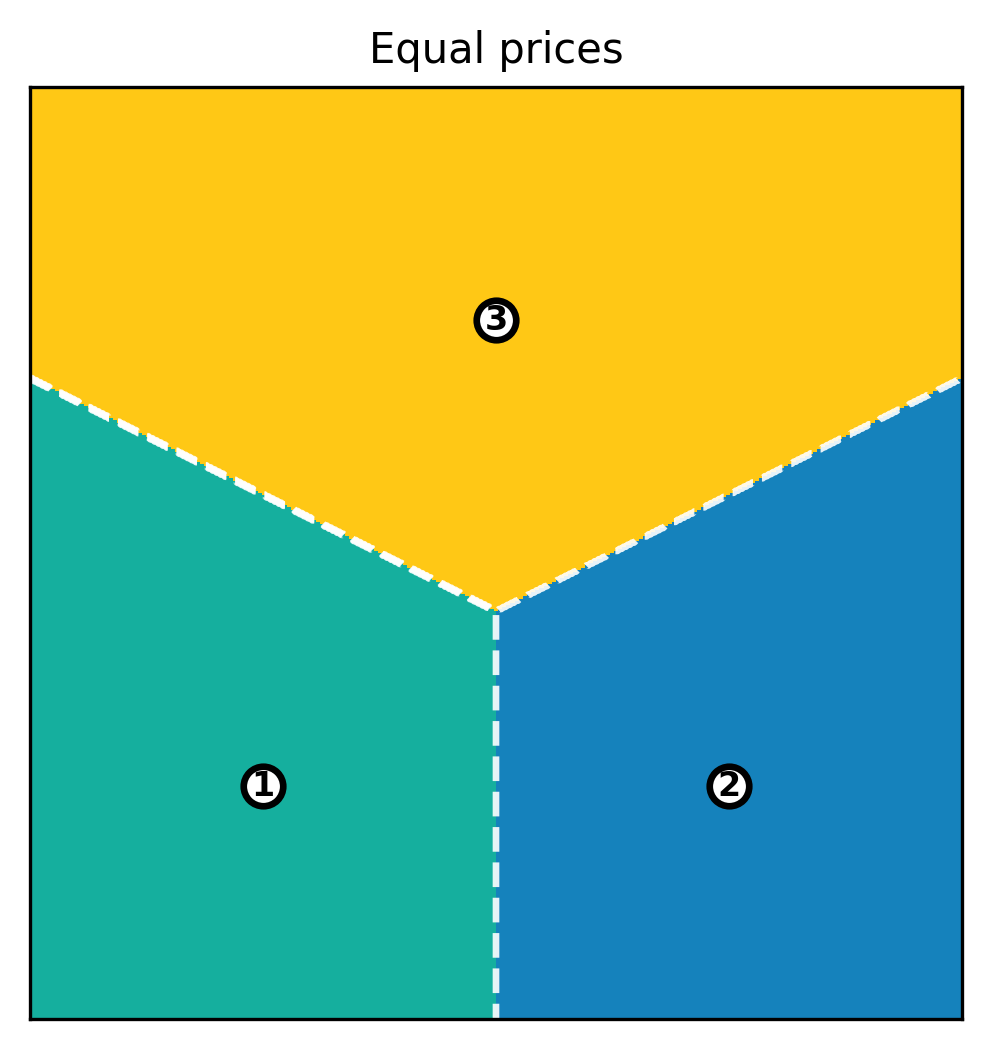
\includegraphics[width=\textwidth]{market_areas_equal_prices.pdf}
  \end{minipage}
  \hfill
  % Second Figure - Price Reduction
  \begin{minipage}{0.45\textwidth}
    \centering
    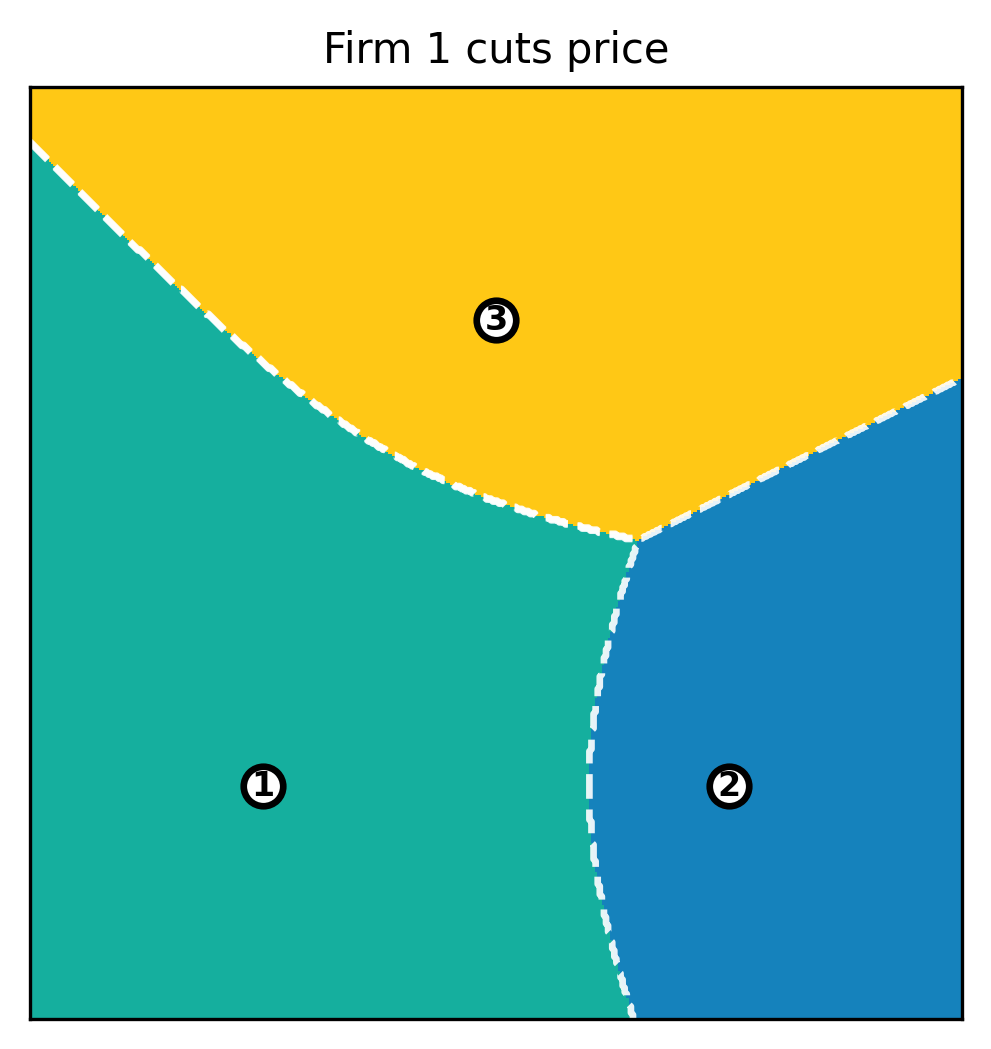
\includegraphics[width=\textwidth]{market_areas_price_reduction.pdf}
  \end{minipage}
  \caption{Market areas defined by the lowest effective price (similar to a weighted Voronoi partition). The left panel shows the case when all firms have the same price. The right panel shows the case when firm 1 lowers its price. Dots mark firm locations.}
  \label{fig:sim1}
\end{figure}

The spatial demand for firm $i$, given the price vector $\mathbf{p}=(p_1,\dots,p_N)$, is:
\begin{equation}
  Q_i(\mathbf{p})
  \;=\;
  \int_S \rho(s)\,(\alpha - \gamma P_i^*(s))\,\mathrm{Prob}\bigl(i\mid s,\mathbf{p}\bigr)\,ds.
\end{equation}

\subsection*{The Optimal Price Problem}

In the static scenario---fixed locations, $N$ firms---each firm chooses its price to maximize profit, taking the locations and prices of rivals as given. Firm $i$ solves:
\begin{equation}
  \Pi_i(\mathbf{p}) \;=\; (p_i - c)\,Q_i(\mathbf{p})
\end{equation}
\begin{equation}
  \max_{p_i \in [c,\overline{p}]} \Pi_i(\mathbf{p})
\end{equation}


We now establish the existence of price equilibria in this spatial competition framework.

\begin{assumption}[Quasi-concavity of profits]\label{ass:qc}
  For each firm $i$ and every fixed $\mathbf{p}_{-i}$, the profit function $\Pi_i(p_i,\mathbf{p}_{-i})$ is quasi-concave in $p_i$ on $[c,\overline{p}]$.
\end{assumption}

\begin{theorem}[Existence of Price Equilibrium]
  \label{thm:existence}
  Under the assumptions above (continuous bounded $\rho$, $\alpha>0, \gamma>0$, $\beta>0$, $t>0$, finite $\overline{p} > c$, compact strategy sets $[c,\overline{p}]$ where $\overline{p}$ ensures $q_i(s)>0$), a logit consumer choice function with linear individual demand, and Assumption \ref{ass:qc}, there exists at least one pure-strategy price equilibrium.
\end{theorem}

\begin{proof}
  (Sketch, following Glicksberg's theorem \citep{glicksberg1952}. The complete proof is given in Appendix \ref{app:existence_proof})

  \noindent
  \textbf{Step 1: Compact, Convex Strategy Sets.}
  Each firm $i$ chooses $p_i$ from the interval $[c, \overline{p}]$, which is compact and convex.

  \noindent
  \textbf{Step 2: Continuity of Profit Functions.}
  $\Pi_i(p_i, \mathbf{p}_{-i})$ is a continuous function of all prices (see Appendix \ref{app:existence_proof}).

  \noindent
  \textbf{Step 3: Quasi-Concavity in Own Price.}
  Assumption \ref{ass:qc} ensures that each firm's objective is quasi-concave in its own price. Appendix \ref{app:existence_proof} provides a sufficient condition in terms of derivatives of $Q_i$.

  \noindent
  \textbf{Step 4: Glicksberg's Fixed Point Theorem.}
  With continuous payoffs, compact convex strategy sets, and quasi-concave payoffs, at least one pure-strategy Nash equilibrium exists.
\end{proof}

The existence proof applies Glicksberg's fixed point theorem, using the properties of continuous payoffs, compact convex strategy sets, and quasi-concavity of profit functions (Assumption \ref{ass:qc}).

While the uniqueness of price equilibria can be established under certain conditions (when the direct own-price sensitivity of demand is sufficiently strong relative to competitive cross-price effects), we focus here on existence, which is sufficient for our analysis of the dynamic entry game.

\section{Dynamic Entry with Fixed Costs}
\label{sec:dynamic}

We now introduce firm entry decisions with fixed costs. Market structure, how many firms enter and where they locate, becomes endogenous.

\subsection*{The Dynamic Entry-Location-Price Game}

Consider an infinite-horizon dynamic game with entry cost $F > 0$ and a common discount factor $\delta \in (0,1)$:

\begin{itemize}
  \item \textbf{Odd periods $(\tau=1,3,\ldots)$ (Entry stage):}
    A potential entrant (firm $N_{\tau-1}+1$) observes the locations $\mathbf{x}_{\tau-1}$ of incumbent firms and decides whether to enter. If entry occurs, the entrant chooses location $x_E^*$ to maximize anticipated profit:
    \begin{equation}
      \max_{x_E \in S} W_E(\mathbf{x}_{\tau-1}, x_E)
    \end{equation}
    where $W_E(\mathbf{x}_{\tau-1},x_E)$ is the potential entrant's continuation value from entering at location $x_E$, defined as the discounted net present value of future price-stage profits minus the fixed cost $F$ under equilibrium continuation play (see Appendix \ref{app:dynamic_entry}).
    Entry occurs if and only if \newline
    $\max_{x_E\in S} W_E(\mathbf{x}_{\tau-1},x_E) > 0$.

  \item \textbf{Even periods $(\tau=2,4,\ldots)$ (Price competition stage):}
    Given locations $\mathbf{x}_\tau$, firms simultaneously set prices, leading to the equilibrium price vector $\mathbf{p}^*(\mathbf{x}_\tau)$ as characterized in Section \ref{sec:static_model}.
\end{itemize}

\begin{assumption}[Regularity of entry values]\label{ass:entry_values}
  For every number of incumbents $N$ and every incumbent location profile $\mathbf{x}_N$, the potential entrant's continuation value
  $W_E(\mathbf{x}_N,\cdot)$ is upper semi-continuous on $S$.
\end{assumption}




\subsection*{Initial Entry: The Monopoly Case}

The first firm to enter the market, for the first two periods, faces no competition and acts as a monopolist. This special case offers analytical solutions for both optimal pricing and location.

\begin{proposition}[Monopoly Price Formula]
  \label{prop:mono_price}
  For a monopolist at location $x_1$, the profit-maximizing price is:
  \begin{equation}
    p_1^*(x_1) = \frac{\alpha}{2\gamma} + \frac{c}{2} - \frac{t \cdot \bar{d}_{\rho}(x_1)}{2},
  \end{equation}

  where $\bar{d_{\rho}}(x_1) = \frac{1}{M}\int_S \rho(s) d(s,x_1) ds$ is the weighted average distance to consumers.
  This solution assumes $\alpha - \gamma c - \gamma t \bar{d}_{\rho}(x_1^*) \geq 0$ to ensure $p_1^*(x_1^*) \geq c$, $p_1^*(x_1^*) \leq \overline{p}$ to guarantee positive demand quantities, and that all consumers in the market consume from the monopolist.
\end{proposition}

\begin{proof}
  For a monopolist at $x_1$, profit is $\Pi(p_1) = (p_1 - c) \int_S \rho(s) (\alpha - \gamma [p_1 + t \cdot d(s,x_1)]) ds$.
  Differentiating with respect to $p_1$ and setting to zero:
  \begin{align*}
    \int_S \rho(s)(\alpha - \gamma [p_1 + t d(s,x_1)])ds + (p_1 - c)\int_S \rho(s)(-\gamma)ds &= 0\\
    M(\alpha - \gamma p_1 - \gamma t \bar{d}_{\rho}(x_1)) - \gamma M(p_1 - c) &= 0\\
    \alpha - \gamma p_1 - \gamma t \bar{d}_{\rho}(x_1) - \gamma p_1 + \gamma c &= 0\\
    \alpha + \gamma c - \gamma t \bar{d}_{\rho}(x_1) &= 2\gamma p_1
  \end{align*}
  Therefore:
  \begin{equation}
    p_1^* = \frac{\alpha}{2\gamma} + \frac{c}{2} - \frac{t \bar{d}_{\rho}(x_1)}{2}
  \end{equation}
  The second derivative $\partial^2 \Pi/\partial p_1^2 = -2\gamma M < 0$ confirms this is a maximum.
\end{proof}

\begin{proposition}[Monopolist Location]
  \label{prop:mono_center}
  The monopolist chooses the location $x_1^*$ that minimizes the weighted average distance to consumers $\bar{d}_{\rho}(x_1)$.
\end{proposition}

\begin{proof}
  Substituting the optimal price into the profit function:
  \begin{equation}
    \Pi(x_1) = \frac{M}{4\gamma}(\alpha - \gamma c - \gamma t \bar{d}_{\rho}(x_1))^2
  \end{equation}
  Assuming $\alpha - \gamma c - \gamma t \bar{d}_{\rho}(x_1) > 0$ (ensuring positive demand), maximizing profit requires minimizing $\bar{d}_{\rho}(x_1)$.
\end{proof}

\begin{remark}
  For uniform consumer density ($\rho(s) = \text{constant}$) in a convex region $S$ and Euclidean distance, the optimal monopolist location solves the (continuous) Fermat--Weber problem, i.e., it is a geometric median of the uniform distribution on $S$. More generally, for arbitrary $\rho$ and distance function $d$, $x_1^*$ is a weighted $1$-median (Fr{\'e}chet median) of the induced distribution.
\end{remark}

\begin{remark}
  The optimal price decreases with average distance: higher transport costs for distant consumers reduce the quantity they demand, so the monopolist lowers the mill price to retain them.
\end{remark}

If the market is initially empty, a necessary condition for the first firm to enter is that the perpetuity value of monopoly profits exceeds the entry cost:
\begin{equation}
  \frac{\Pi(x_1^*)}{1-\delta} > F
\end{equation}

This condition is exact when no further entry occurs; in general the first entrant's continuation value depends on subsequent entry (see Appendix \ref{app:dynamic_entry}).
If entry occurs, the first entrant locates at $x_1^*$ and sets price $p_1^*(x_1^*)$ as characterized above in the initial monopoly phase.

\subsection*{Equilibrium Analysis with Multiple Firms}

After the first entry, subsequent firms may enter sequentially, each choosing their optimal location given the existing configuration of incumbents.

\begin{theorem}[Existence of SPNE with Entry]
  \label{thm:existence_entry}
  Under the assumptions of our model, with a positive fixed entry cost $F > 0$, a common discount factor $\delta \in (0,1)$, assuming the price equilibrium exists for any configuration of firms, and Assumption \ref{ass:entry_values}, there exists a subgame perfect Nash equilibrium (SPNE) in the infinite-horizon entry-location-price game.
\end{theorem}

\begin{proof}
  See Appendix \ref{app:dynamic_entry}.
\end{proof}

\begin{theorem}[Non-Uniqueness of SPNE with Entry]
  \label{thm:non_uniqueness_entry}
  The entry-location-price game generally admits multiple subgame perfect Nash equilibria, distinguished by different numbers of firms, different location configurations, or both.
\end{theorem}

\begin{proof}
  See Appendix \ref{app:dynamic_entry}.
\end{proof}

An equilibrium market structure exists, but typically not a unique one. Multiplicity arises from four sources: multiple optimal locations for each entrant, path dependence in sequential entry decisions, strategic entry deterrence by incumbents, and the integer constraint on the number of firms. As a result, comparative statics in $N^*$ are stepwise: parameter changes may leave $N^*$ unchanged until a threshold is crossed.

\subsection*{Equilibrium Properties}

\begin{proposition}[Market Structure Properties]
  \label{prop:market_structure}
  The equilibrium number of firms $N^*$ in the entry-location-price game with fixed cost $F$:
  \begin{enumerate}
    \item Decreases with $F$ (higher entry costs lead to fewer firms)
    \item Increases with market size $M$ (larger markets support more firms)
    \item Decreases with parameters that intensify price competition ($\beta$ and $\gamma$)
    \item Increases with parameters that soften price competition (larger $t$)
  \end{enumerate}
  \medskip
  \noindent\emph{Note.} Since $N$ must be an integer, these changes occur in discrete steps (e.g., $N^*$ remains constant for a range of $F$ before jumping down).
\end{proposition}

\begin{proof}
  See Appendix \ref{app:dynamic_entry}.
\end{proof}

Higher entry costs and stronger price competition reduce the number of firms that can earn non-negative profits; larger markets and higher transport costs work in the opposite direction by sustaining markups.

\begin{proposition}[Comparative Statics]
  \label{prop:comparative}
  Assuming a price equilibrium exists for any configuration of firms, we obtain the following comparative statics:

  \begin{enumerate}
    \item Increasing $\beta$ (more price-sensitive consumer choice) generally leads to \emph{lower} equilibrium prices $p_i^*$.
    \item Increasing $\gamma$ (higher price sensitivity of demand) generally leads to \emph{lower} equilibrium prices $p_i^*$.
    \item Increasing $t$ (higher transportation costs) tends to \emph{increase} equilibrium prices $p_i^*$ by softening competition through greater spatial differentiation.
    \item Increasing $\alpha$ (higher base demand) generally leads to \emph{higher} equilibrium prices $p_i^*$.
  \end{enumerate}
\end{proposition}

\begin{proof}
  See Appendix \ref{app:comparative_statics}.
\end{proof}

Higher $\beta$ and $\gamma$ make consumers more price-responsive, so competition intensifies and prices fall. Higher transportation costs ($t$) increase spatial differentiation and allow firms to sustain higher prices. Higher base demand ($\alpha$) raises willingness to pay and pushes prices up.

\section{Relationship to Classical Models}
\label{sec:classical}

Our framework connects to classical spatial competition models as limiting cases. In particular, under unit demand and in the deterministic choice limit $\beta\to\infty$, market areas coincide with those in Hotelling's linear city and Salop's circular city.

\subsection{Hotelling's Linear City}

\begin{proposition}[Hotelling Special Case]
  \label{prop:hotelling}
  Let $S = [0,1]\times\{0\}$, $\rho(s)=1$, $d(s,x)=|s-x|$, and $N=2$. Assume unit demand and full market coverage. Then as $\beta\to\infty$, consumer choices become deterministic and market areas become intervals defined by the lowest effective price $P_i^*(s)=p_i+t|s-x_i|$, recovering Hotelling's linear city.
\end{proposition}

\begin{proof}
  As $\beta \to \infty$, $\mathrm{Prob}(i|s,\mathbf{p}) \to 1$ for the firm with the lowest $P_i^*(s)$. With unit demand, $Q_i(\mathbf{p}) \to \text{length}(V_i(\mathbf{p}))$, where $V_i(\mathbf{p})$ is the region where firm $i$ offers the lowest effective price. This recovers Hotelling's model.
\end{proof}

\subsection{Salop's Circular City}

\begin{proposition}[Salop Special Case]
  \label{prop:salop}
  Let $S$ be a circle of circumference $L$, $\rho(s)=1/L$, and let $d(s,x)$ be arc distance. Assume unit demand and full market coverage. As $\beta\to\infty$, market areas become arc segments, recovering Salop's circular city.
\end{proposition}

\begin{proof}
  Similar to the Hotelling case, $Q_i(\mathbf{p}) \to \text{length}(V_i(\mathbf{p}))/L$ as $\beta \to \infty$, recovering Salop's model.
\end{proof}

\begin{remark}
  Both special cases require $\beta \to \infty$ (deterministic consumer choice) and unit demand. Probabilistic demand ($\beta < \infty$) combined with a linear quantity response allows for smoother substitution and a non-trivial quantity margin, both absent from the classical cases. For arbitrary convex distance functions $d$, our model converges to a generalized Voronoi-Hotelling model as $\beta \to \infty$.
\end{remark}


\section{Equilibrium Analysis and Simulations}
\label{sec:simulations}

While the model guarantees the existence of a price equilibrium, its specific characteristics for $N > 1$ are analytically intractable. We therefore use numerical simulations to illustrate the geometry of market areas, the effect of heterogeneous consumer density, and the sequential entry mechanism of Section \ref{sec:dynamic}. Unless otherwise stated, the simulations are conducted in a square market $S = [0,1]^2$ with Euclidean distance. Integrals are approximated on a uniform grid and equilibrium prices are computed by best-response iteration. The full numerical implementation and baseline parameterization are reported in Appendix \ref{app:numerics}.

As a regularity diagnostic connected to Assumption \ref{ass:R}, for each scenario we compute the curvature ratio $\eta_i(\mathbf{p}^*)$ at the computed equilibrium prices and a conservative own-price scan. The resulting values are reported in Appendix \ref{app:numerics} (Table \ref{tab:eta_diagnostics}).

We first illustrate how the consumer choice sensitivity $\beta$ governs the sharpness of market areas. Figure \ref{fig:sim2} fixes three firm locations and compares the equilibrium outcome for increasing values of $\beta$. For low $\beta$ the market shares are diffuse, while for high $\beta$ the induced partition becomes nearly deterministic and approaches the Voronoi diagram.

The effect of $\beta$ on equilibrium prices and profits need not be monotone. Economically, $\beta$ controls the strength of substitution across firms through the logit term: letting $L_i(s,\mathbf{p})=\mathrm{Prob}(i\mid s,\mathbf{p})$, we have $\partial L_i/\partial p_i = -\beta\,L_i(1-L_i)$. When $\beta$ is small, shares are close to $1/N$ and weakly responsive to prices, so a unilateral price increase does not shift much demand to rivals and equilibrium markups can be high. As $\beta$ rises to moderate values, substitution becomes stronger (both because of the higher $\beta$ and because $L_i(1-L_i)$ is sizeable), intensifying price competition and reducing markups. For very large $\beta$, however, choice becomes nearly deterministic: away from the boundaries between firms, $L_i$ is close to $0$ or $1$ so $L_i(1-L_i)\approx 0$, and competitive pressure is concentrated on a small set of consumers near indifference loci. In such highly segmented configurations, firms may regain some local market power inside their (almost) Voronoi cells, so equilibrium prices can vary little or even increase slightly with further increases in $\beta$.

\begin{figure}
  \centering
  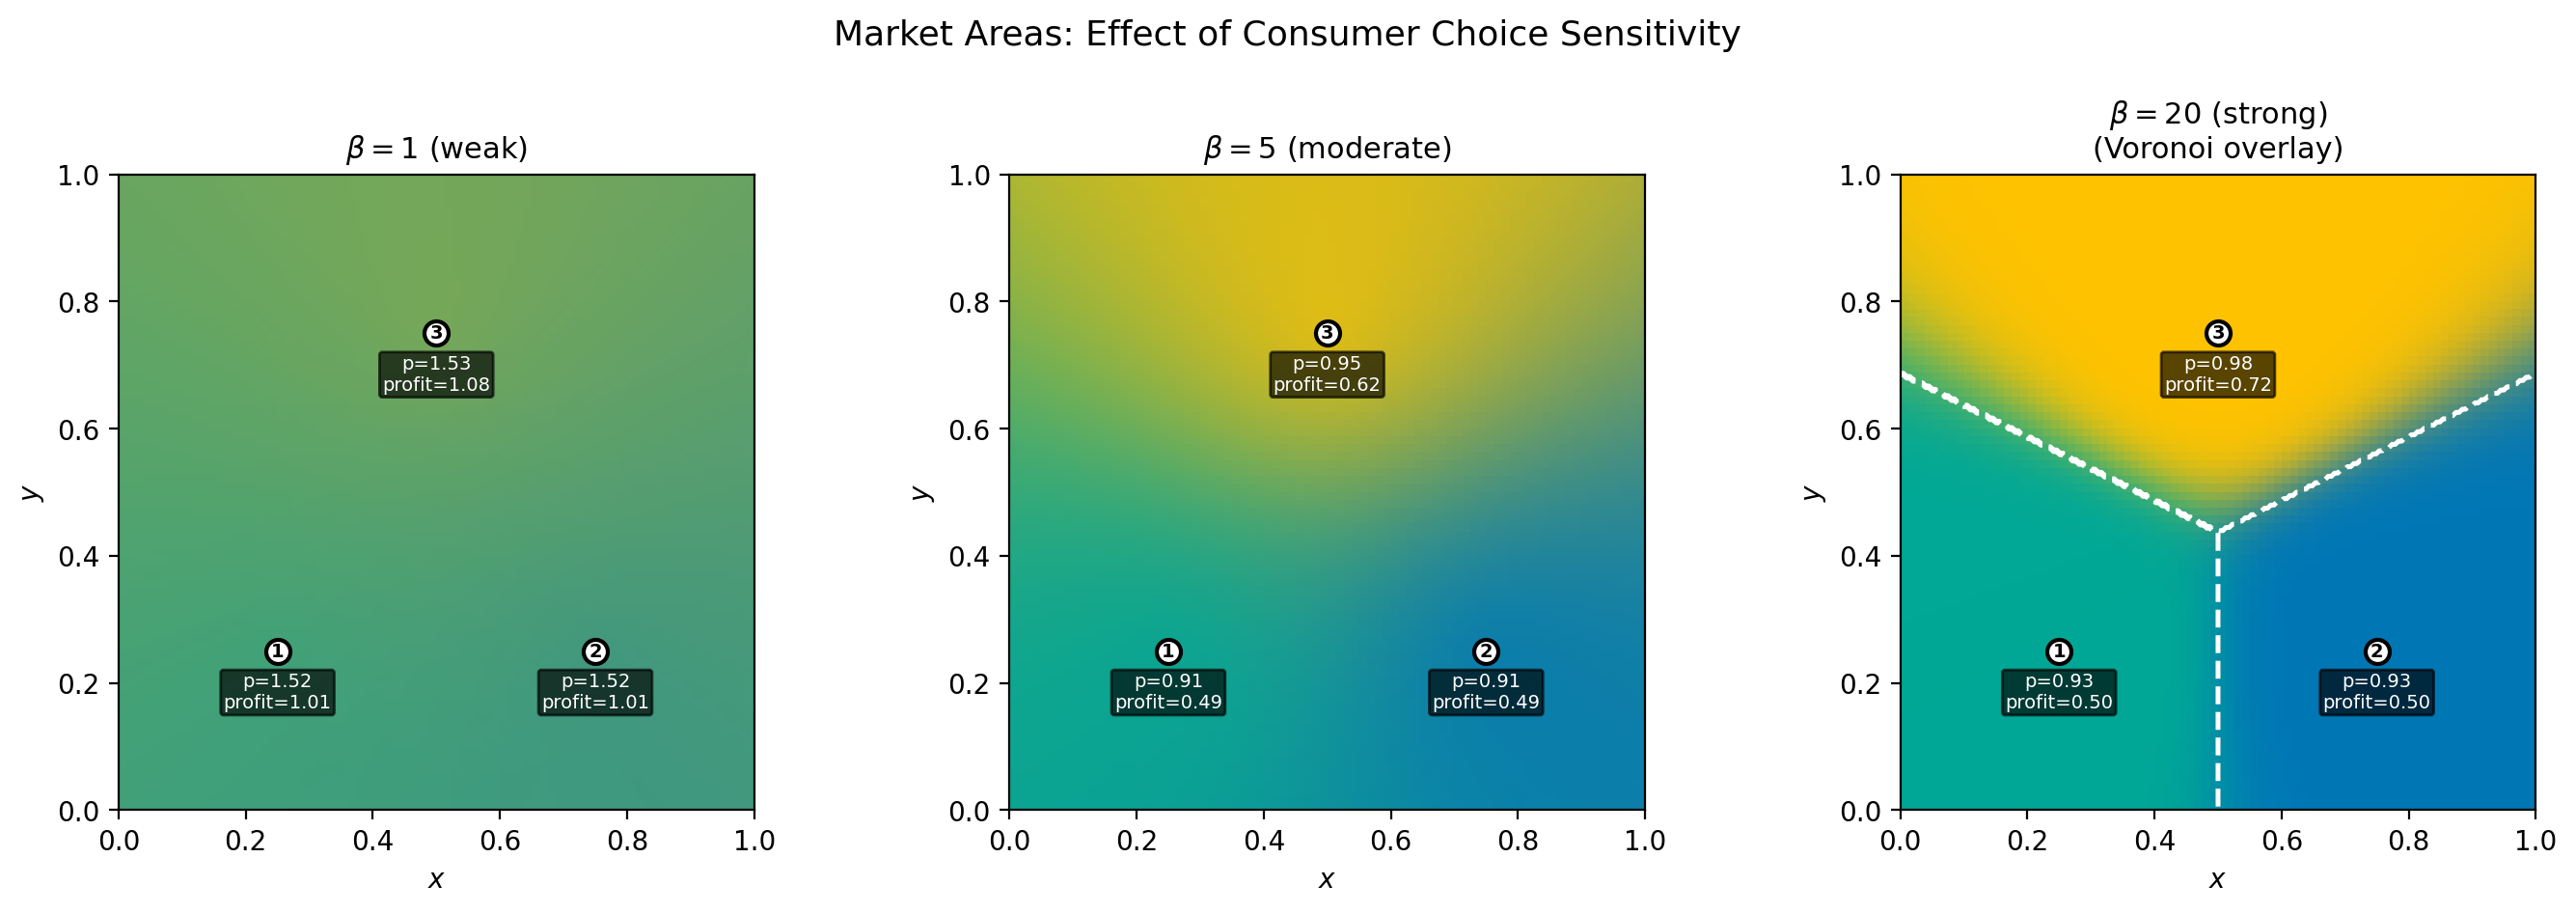
\includegraphics[width=0.98\linewidth]{figures_toy/fig1_beta_comparison.pdf}
  \caption{Effect of consumer price sensitivity $\beta$ on market areas (uniform density, three firms at fixed locations). Colored regions represent market shares; dashed lines overlay the Voronoi partition. As $\beta$ increases, choice becomes more deterministic and market areas converge to Voronoi cells; equilibrium prices fall sharply from low to moderate $\beta$ and then vary little at higher $\beta$ in this configuration. Labels report equilibrium prices and profits.}
  \label{fig:sim2}
\end{figure}

Consider now the dynamic model. In the first two periods there is only one firm in the economy which will choose location first and then its price. The first firm is unaware whether new firms will enter the market and will behave in this initial phase as a monopolist.
We derived in Proposition \ref{prop:mono_price} that the monopolist's optimal \emph{mill price} decreases linearly in the transport cost, because higher $t$ raises delivered prices and reduces quantities under linear demand. In particular, at the optimal location $x_1^*$ we have
\[
  p_1^*(x_1^*) \;=\; \frac{\alpha}{2\gamma} + \frac{c}{2} \;-\; \frac{t}{2}\,\bar d_\rho(x_1^*),
\]
While the mill price decreases in $t$, the corresponding average delivered price paid by consumers increases:
\[
  \bar P_1^* \;\equiv\; p_1^*(x_1^*) + t\,\bar d_\rho(x_1^*).
\]
Both objects converge to the standard non-spatial monopoly price with linear demand,
$p_m=\frac{\alpha}{2\gamma}+\frac{c}{2}$, as $t\to 0$. Figure \ref{fig:sim3} plots these comparative statics.

\begin{figure}[h]
  \centering
  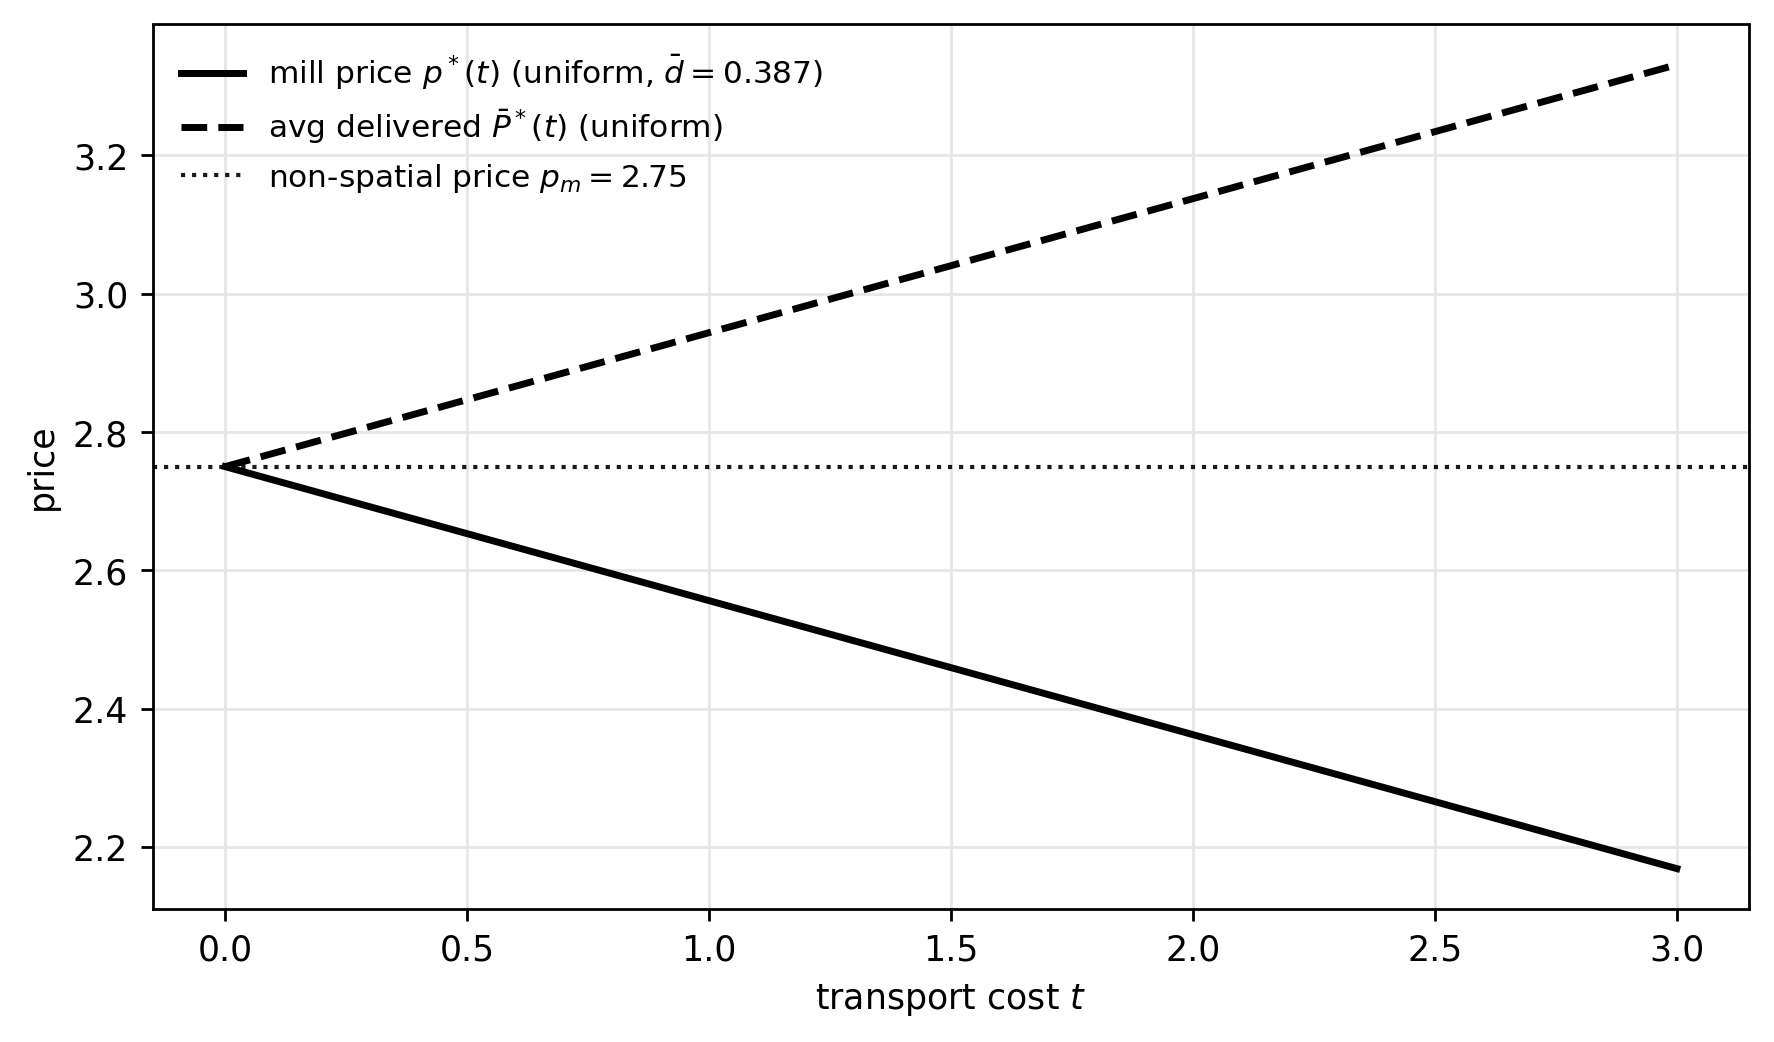
\includegraphics[width=0.9\linewidth]{figures_toy/fig_monopoly_mill_vs_delivered.pdf}
  \caption{Monopolist case. The optimal mill price $p_1^*(x_1^*)$ (solid) decreases linearly in the transport cost $t$, while the average delivered price $\bar P_1^*$ (dashed) increases linearly. The dotted line marks the non-spatial monopoly price $p_m=\frac{\alpha}{2\gamma} + \frac{c}{2}$, which both objects converge to as $t\to 0$.}
  \label{fig:sim3}
\end{figure}

After the first and second periods, new firms can choose to enter the market until entry is no longer profitable.

\begin{comment}
    Figure shows the final equilibrium before it ends at the xth period because no firm found it profitable to enter.
\end{comment}
We next illustrate the effect of heterogeneous consumer density on equilibrium prices and market shares. Figure \ref{fig:sim4} considers a triopoly with fixed locations and compares the equilibrium under uniform density to a market with a single demand peak. The firm located close to the peak captures a larger market share and can profitably set a higher price.

\begin{figure}
  \centering
  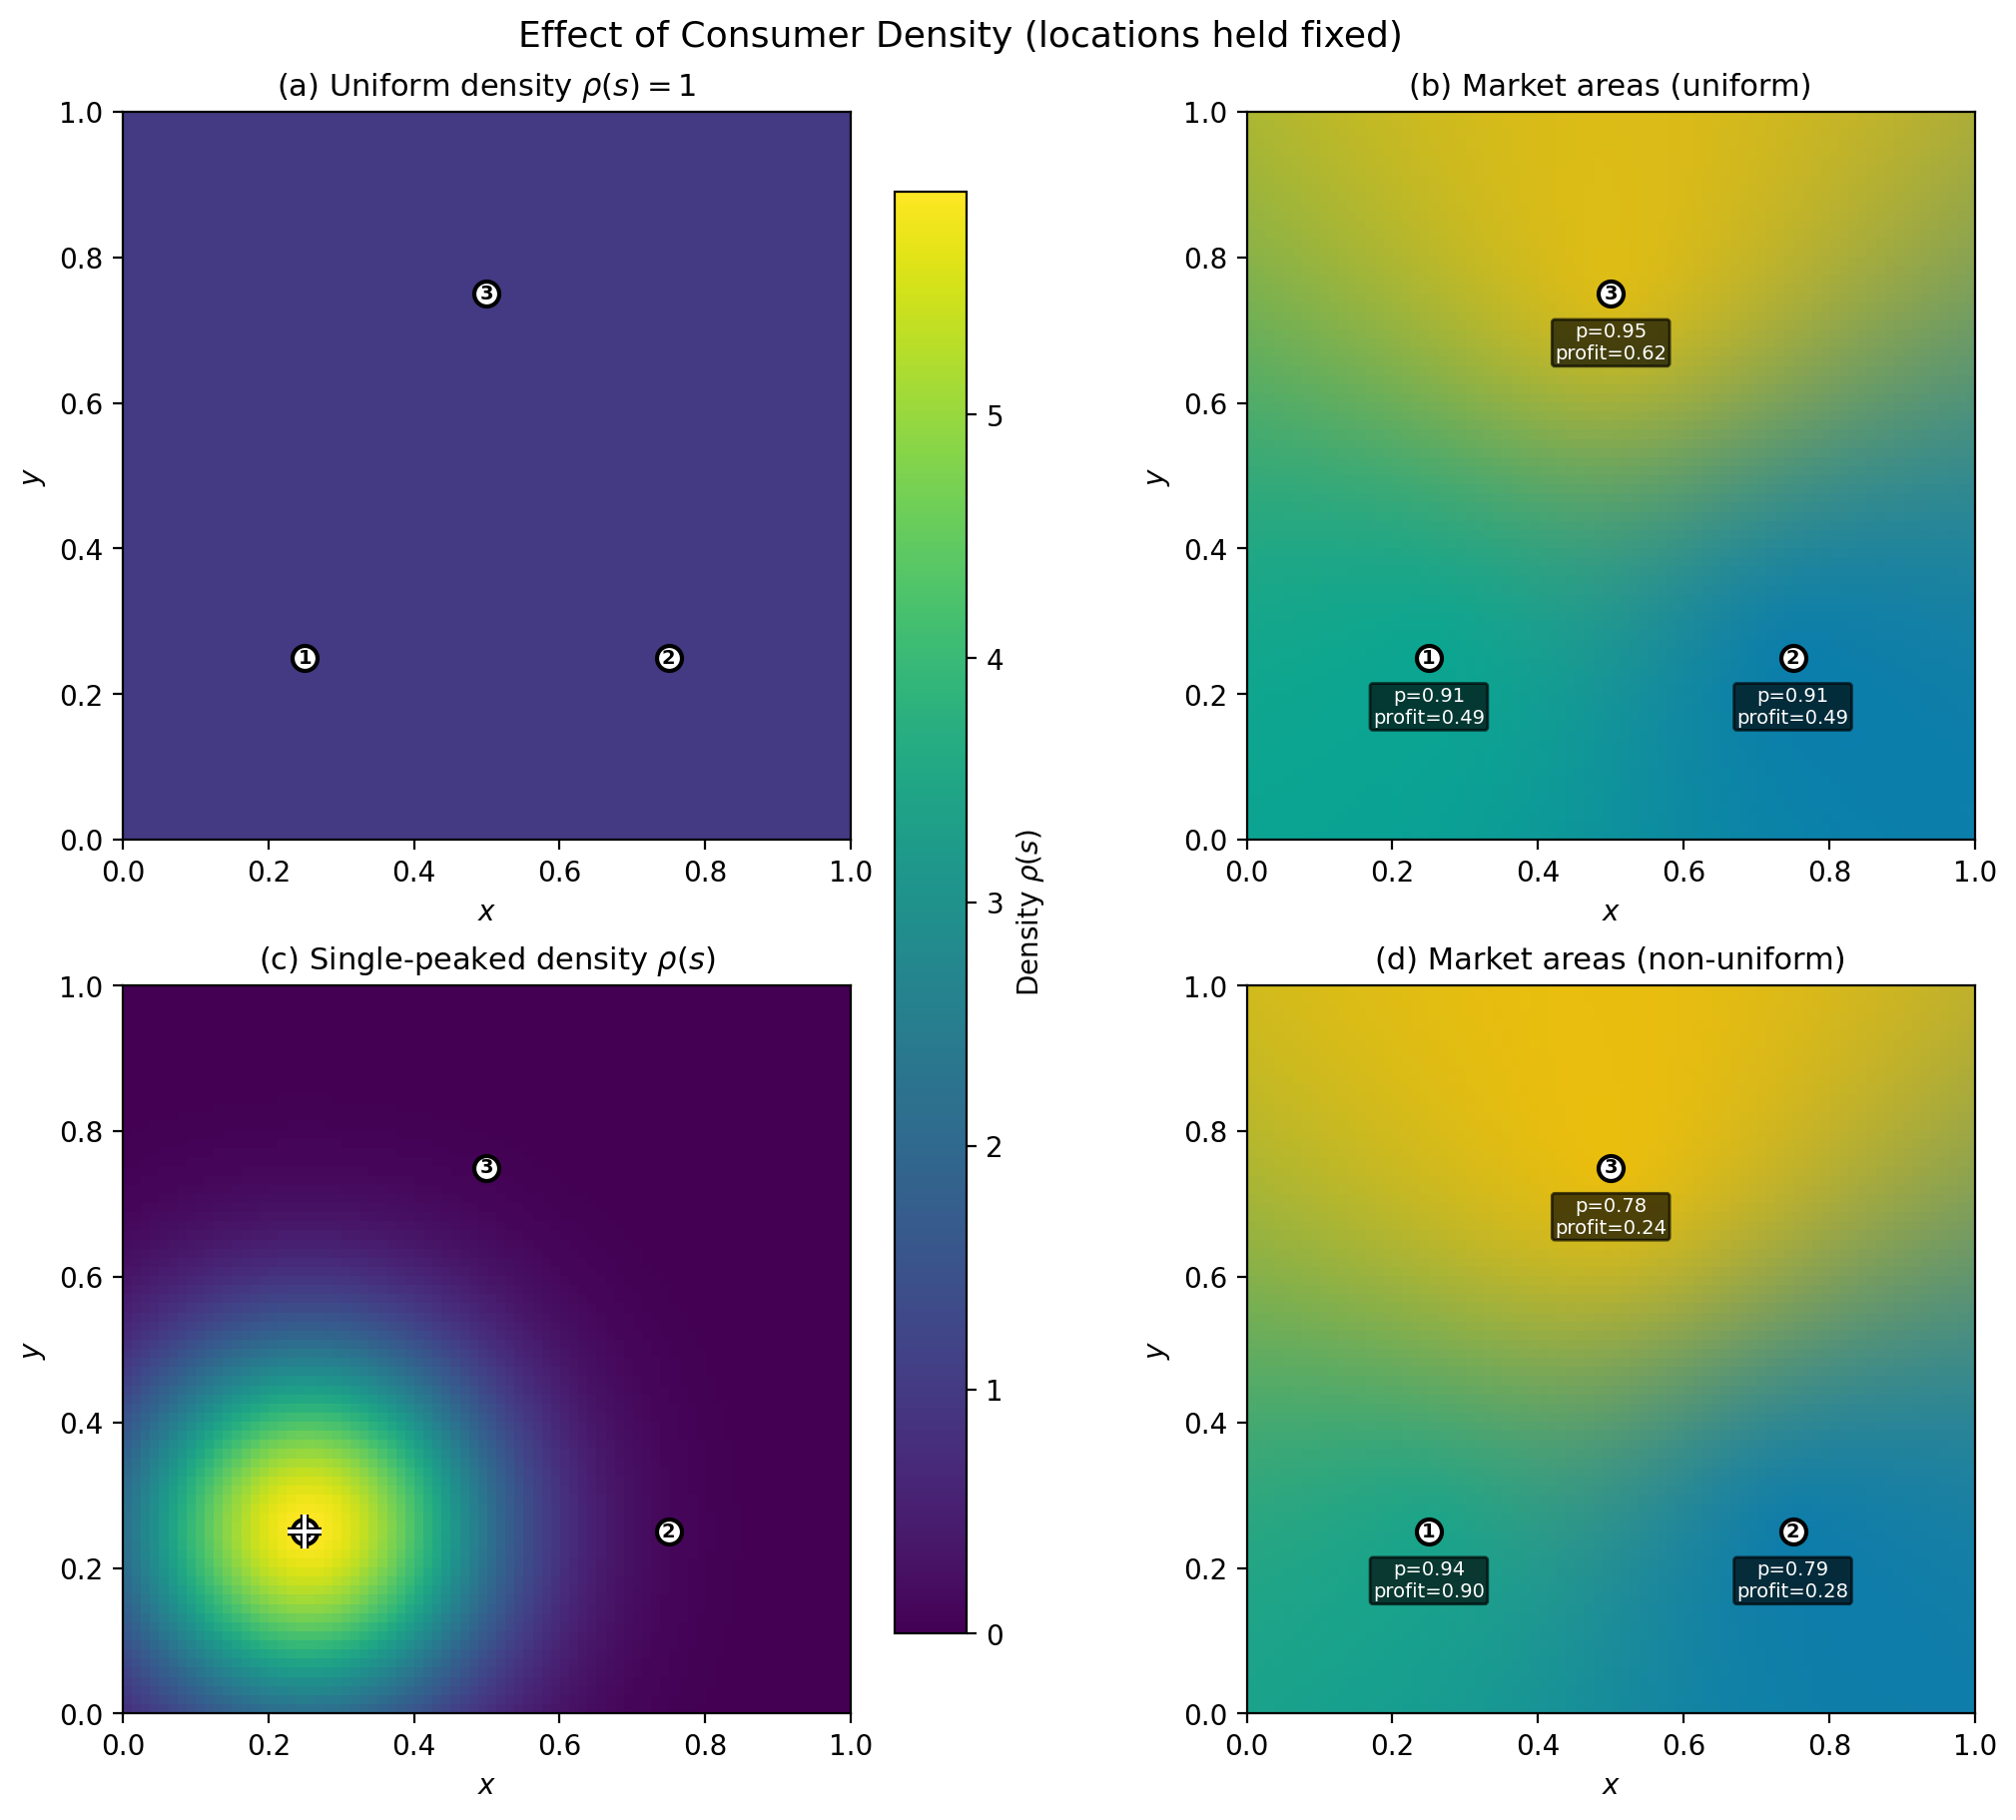
\includegraphics[width=0.98\linewidth]{figures_toy/fig2_density.pdf}
  \caption{Effect of heterogeneous consumer density holding firm locations fixed (to isolate the role of $\rho$ in price competition). The left column reports the consumer density (uniform versus single-peaked, normalized to integrate to one; peak marked by ``+''). The right column reports the corresponding equilibrium market shares. Labels report equilibrium prices and profits.}
  \label{fig:sim4}
\end{figure}

Finally, Figure \ref{fig:sim5} illustrates a sequential entry path under uniform density and high $\beta$. Starting from a monopoly, each entrant chooses a location to maximize its post-entry profit on a finite candidate grid, and prices adjust to the static equilibrium each period. The top panels display selected stages of the entry path; the bottom panel plots the implied equilibrium number of firms $N^*(F)$ as a function of the entry cost $F$ for this realized sequence of entry profits. Additional numerical illustrations are reported in Appendix \ref{app:numerics}.

\begin{figure}
  \centering
  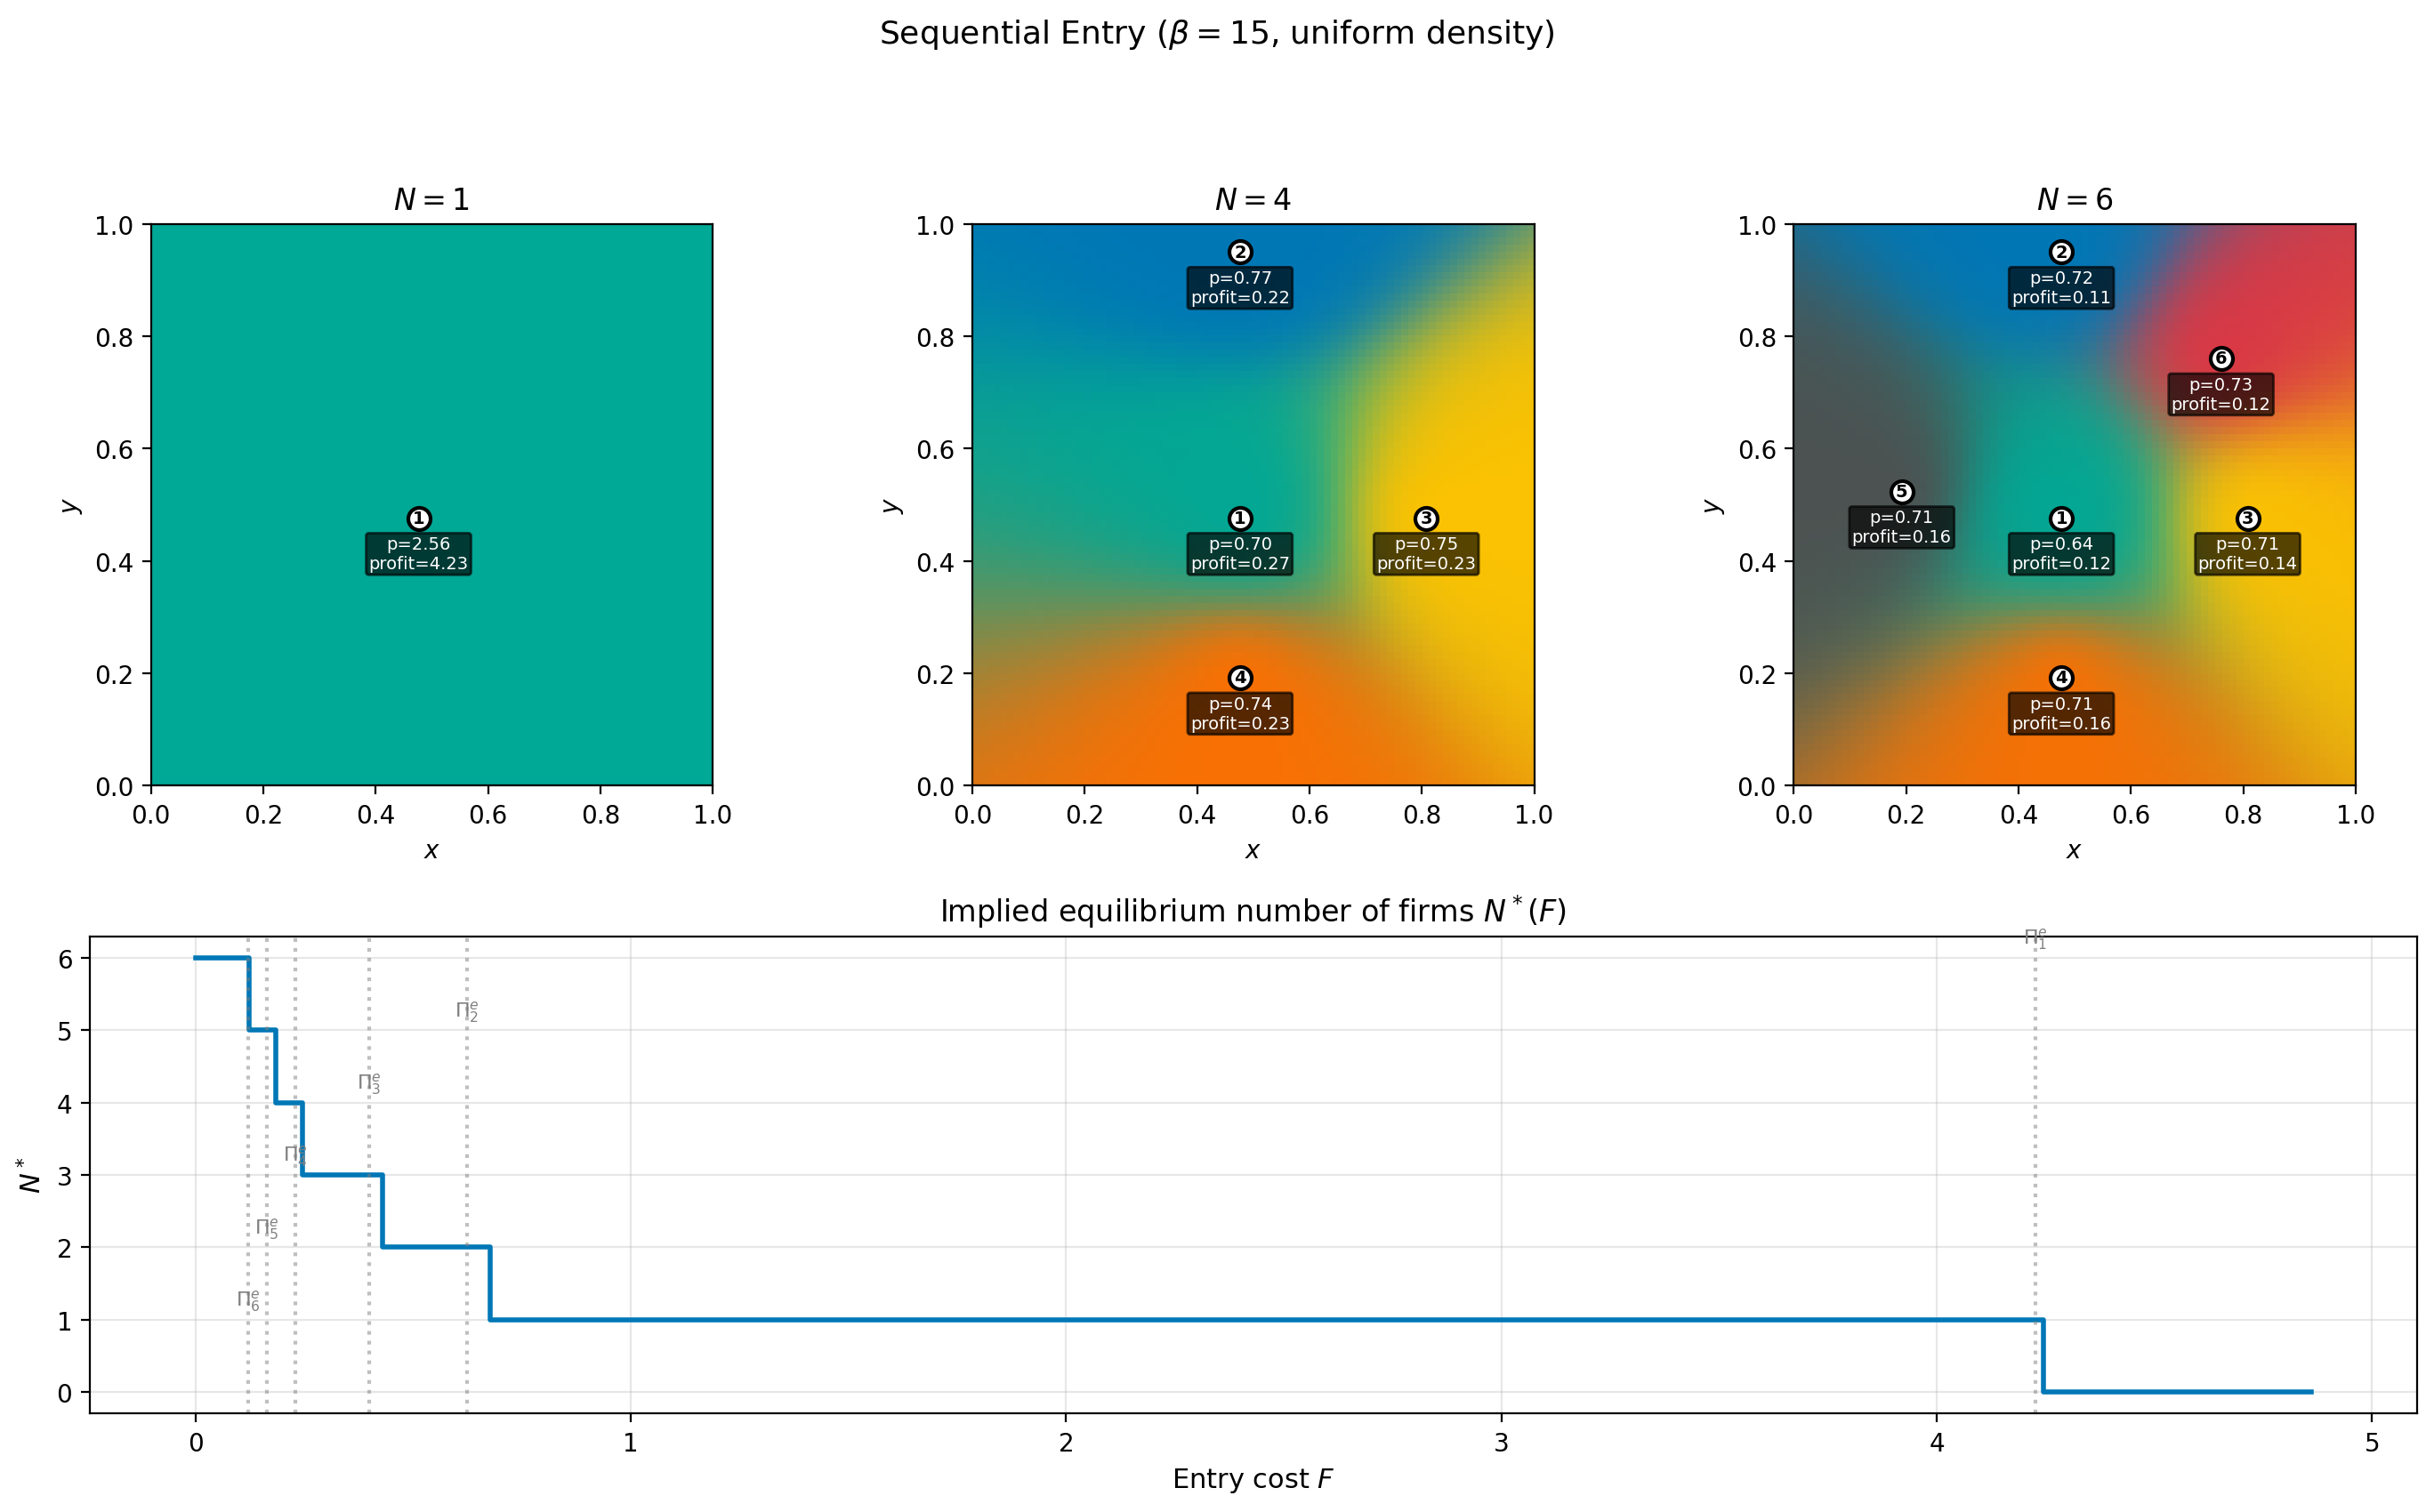
\includegraphics[width=0.98\linewidth]{figures_toy/fig3_entry.pdf}
  \caption{Sequential entry illustration under uniform density ($\beta=15$). In each period a potential entrant chooses the location that maximizes its post-entry profit on a candidate grid; prices are the static equilibrium prices given locations. The bottom panel plots the entry threshold $N^*(F)$ implied by the sequence of entry profits along this path. Labels report equilibrium prices and profits.}
  \label{fig:sim5}
\end{figure}


\subsection{Spatial Differentiation: Agglomeration vs. Dispersion}

The simulations also address where firms locate relative to each other, the classic minimum vs.\ maximum differentiation question \citep{daspremont1979hotelling, depalma85}. Two forces compete: a ``demand pull'' draws firms toward density peaks, while a ``competitive push'' drives them apart to reduce price competition. Which dominates depends chiefly on the consumer choice sensitivity $\beta$.

\begin{remark}[Spatial Differentiation Regimes (Numerical)]
  \label{rem:differentiation}
  In our simulations, we observe two regimes:
  \begin{enumerate}
    \item \textbf{Agglomeration Regime:} For sufficiently low values of $\beta$, firms tend to cluster.
    \item \textbf{Dispersion Regime:} For sufficiently high values of $\beta$ and transport cost $t$, firms tend to disperse to soften price competition.
  \end{enumerate}
\end{remark}

Figure \ref{fig:differentiation} illustrates these regimes computationally in a market with a central density peak. Firms enter sequentially. With low $\beta$, the demand-pull dominates and entrants locate close to the density peak (Panel a). With high $\beta$ and $t$, the incentive to avoid head-to-head price competition dominates and firms spread out despite the density peak (Panel b).

\begin{figure}
  \centering
  % Panel A: Agglomeration Regime
  \begin{minipage}{0.48\textwidth}
    \centering
    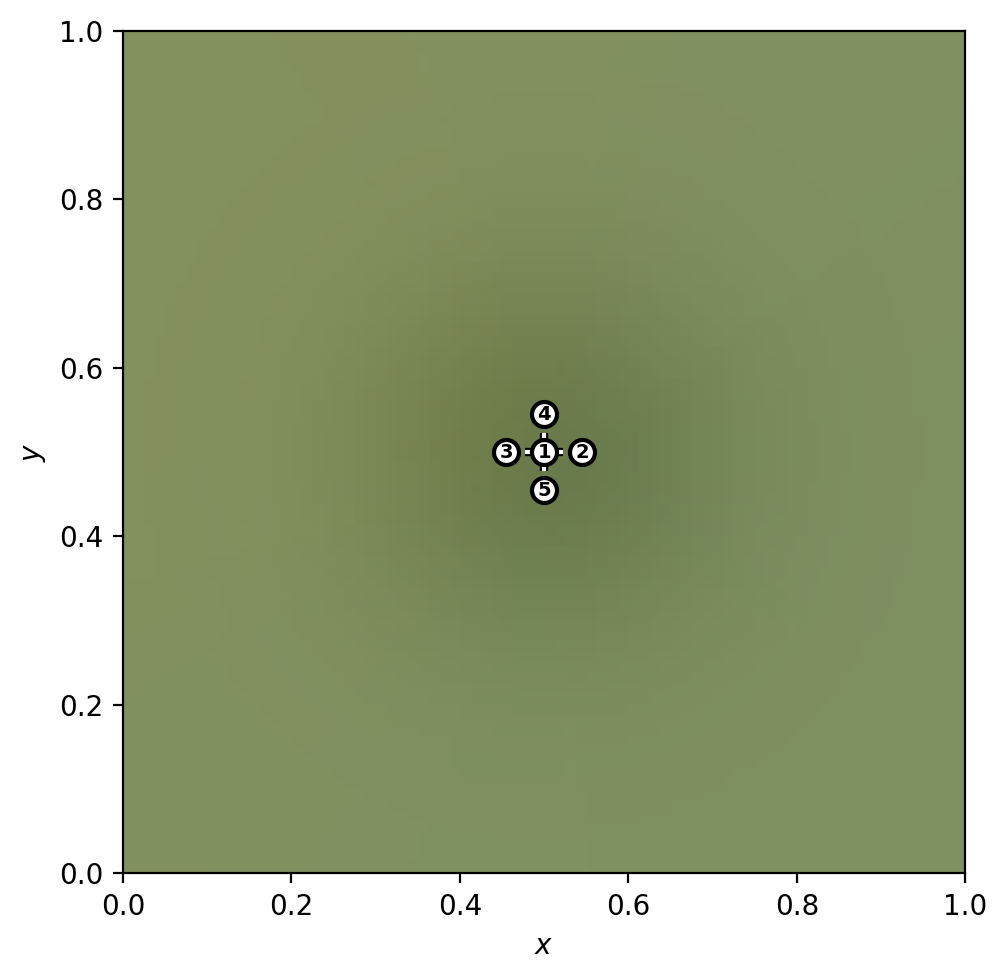
\includegraphics[width=\textwidth]{aggregation.pdf}
    \caption*{(a) Agglomeration Regime (Low $\beta$)}
  \end{minipage}
  \hfill % This creates space between the two minipages
  % Panel B: Dispersion Regime
  \begin{minipage}{0.48\textwidth}
    \centering
    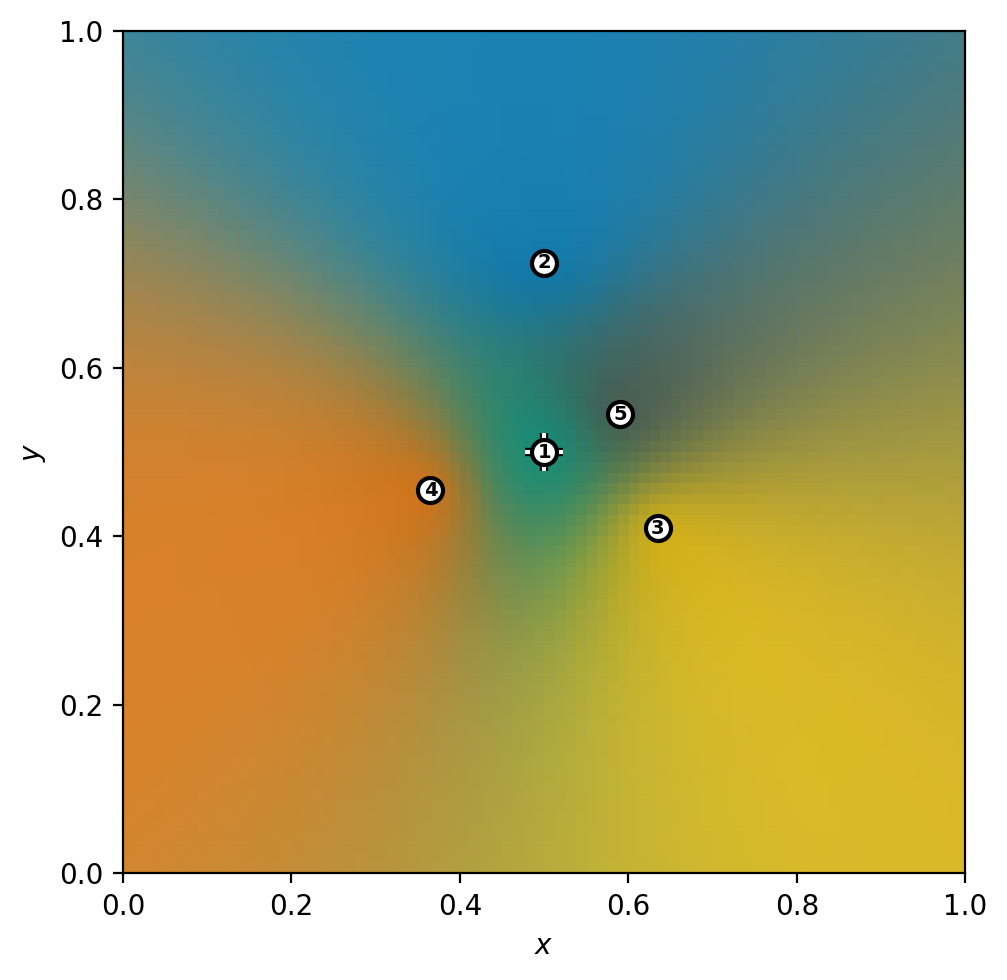
\includegraphics[width=\textwidth]{differentiation.pdf}
    \caption*{(b) Dispersion Regime (High $\beta$, high $t$)}
  \end{minipage}
  \caption{Equilibrium locations for five firms under different differentiation regimes in a market with a central density peak. The background shading indicates consumer density.}
  \label{fig:differentiation}
\end{figure}

\section{Conclusion}
\label{sec:conclusion}

This paper took Hotelling's framework to two dimensions, allowed for non-uniform consumer density, and introduced probabilistic (logit) choice. We proved that price equilibria exist in the static game and that subgame perfect Nash equilibria exist in the dynamic entry game with fixed costs, though generally multiple ones, due to location multiplicity and path dependence. The monopoly case admits closed-form solutions: the optimal location minimizes the weighted average distance to consumers, and the optimal price decreases linearly with that distance.

The simulations show that the same model can generate both firm clustering and dispersion. When consumer price sensitivity is low, the pull toward demand peaks dominates and firms agglomerate. When sensitivity is high and transport costs are large, the incentive to avoid head-to-head competition dominates and firms spread out.

The model connects to Hotelling's line and Salop's circle as limiting cases under deterministic choice ($\beta \to \infty$) and unit demand. The two-dimensional, probabilistic version is more general but also harder to analyze: numerical methods fill the gap for multi-firm configurations.

The framework can be brought to data when consumer locations and firm prices are observed; the monopoly case in particular may be tractable with retail scanner data.

\newpage
\appendix

\section{Numerical Implementation and Additional Results}
\label{app:numerics}

This appendix describes the numerical implementation used to generate the figures in Section \ref{sec:simulations} and reports additional numerical illustrations.

\subsection{Numerical Setup}
\begin{description}
  \item[Market, grids, and densities.] We set $S=[0,1]^2$ and approximate integrals on a uniform $n\times n$ quadrature grid (baseline $n=80$). For non-uniform densities, we normalize $\rho$ to have unit mass, $\int_S \rho(s)\,ds = 1$, so that profit magnitudes are comparable across density scenarios.

  \item[Price equilibrium solver.] Given firm locations, equilibrium prices are computed by damped best-response iteration over the compact set $[c,\overline{p}]^N$ (damping $0.5$, tolerance $10^{-9}$, maximum $500$ iterations).

  \item[Entry algorithm (illustrative).] In sequential-entry figures, an entrant searches over an $m\times m$ candidate grid (baseline $m=20$) and enters at the location that maximizes its post-entry profit given incumbents; prices then adjust to the static equilibrium. Because the entrant objective can be flat in symmetric configurations, this procedure induces deterministic tie-breaking and can generate path dependence (Figure \ref{fig:app_multiplicity}).

  \item[Baseline parameters.] Unless otherwise stated we use $(\alpha,\gamma,t,c,\overline{p})=(5,1,1,0.5,3.5)$ and vary $\beta$ as indicated in each figure.
\end{description}

\subsection{Additional Numerical Illustrations}
Figures \ref{fig:app_compstat}--\ref{fig:app_multiplicity} provide complementary numerical illustrations for the comparative statics and the sequential entry mechanism discussed in the main text.

\paragraph{Comparative statics}
Figure \ref{fig:app_compstat} reports numerical comparative statics of equilibrium prices with respect to $(\beta,\gamma,t,\alpha)$, holding firm locations fixed under uniform density. This complements Proposition \ref{prop:comparative} and the proof sketch in Appendix \ref{app:comparative_statics}.

\begin{figure}
  \centering
  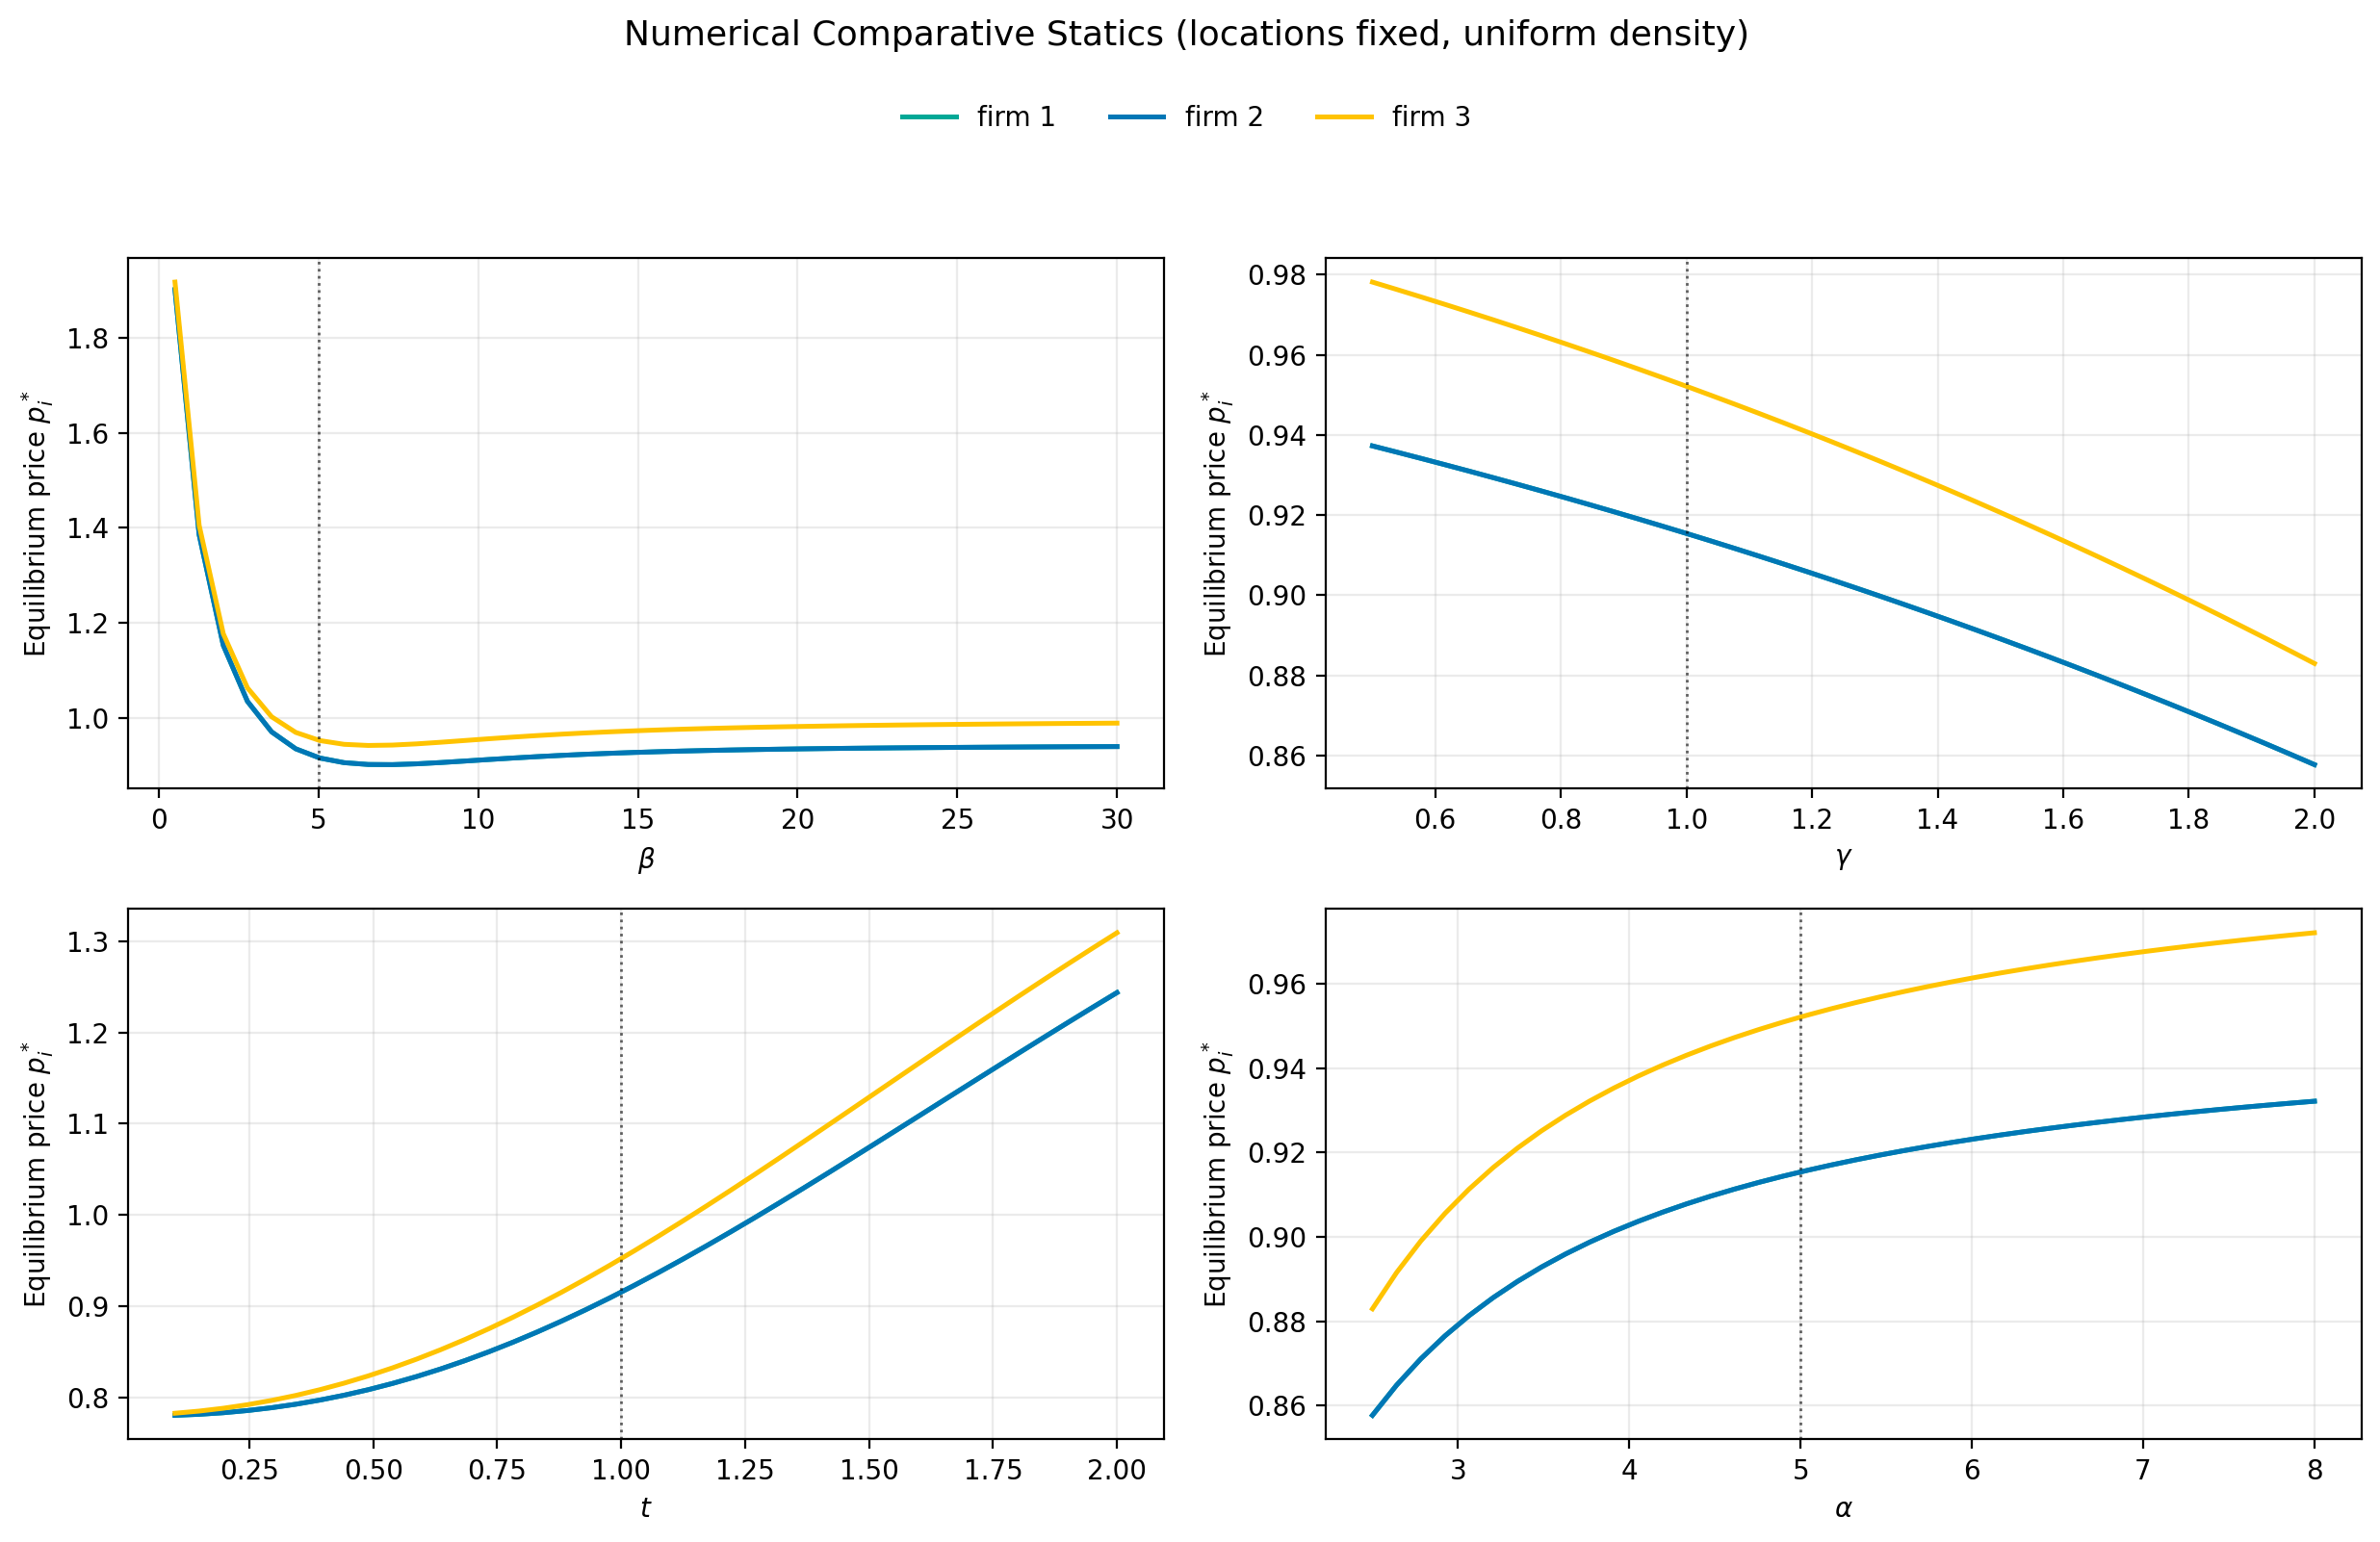
\includegraphics[width=0.95\linewidth]{figures_toy/fig4_compstat.pdf}
  \caption{Numerical comparative statics for equilibrium prices under uniform density and fixed locations. Each panel varies one parameter while holding the others at the baseline values.}
  \label{fig:app_compstat}
\end{figure}

\paragraph{Entry costs and discounting}
To illustrate how discounting rescales the entry threshold, Figure \ref{fig:app_nstar_delta} plots $N^*(F)$ for different $\delta$ under the heuristic rule $\Pi^e/(1-\delta)>F$, where $\Pi^e$ denotes the entrant's post-entry profit along a baseline entry path. This is not the equilibrium condition of the full dynamic game, but it helps interpret the role of $\delta$.

\begin{figure}
  \centering
  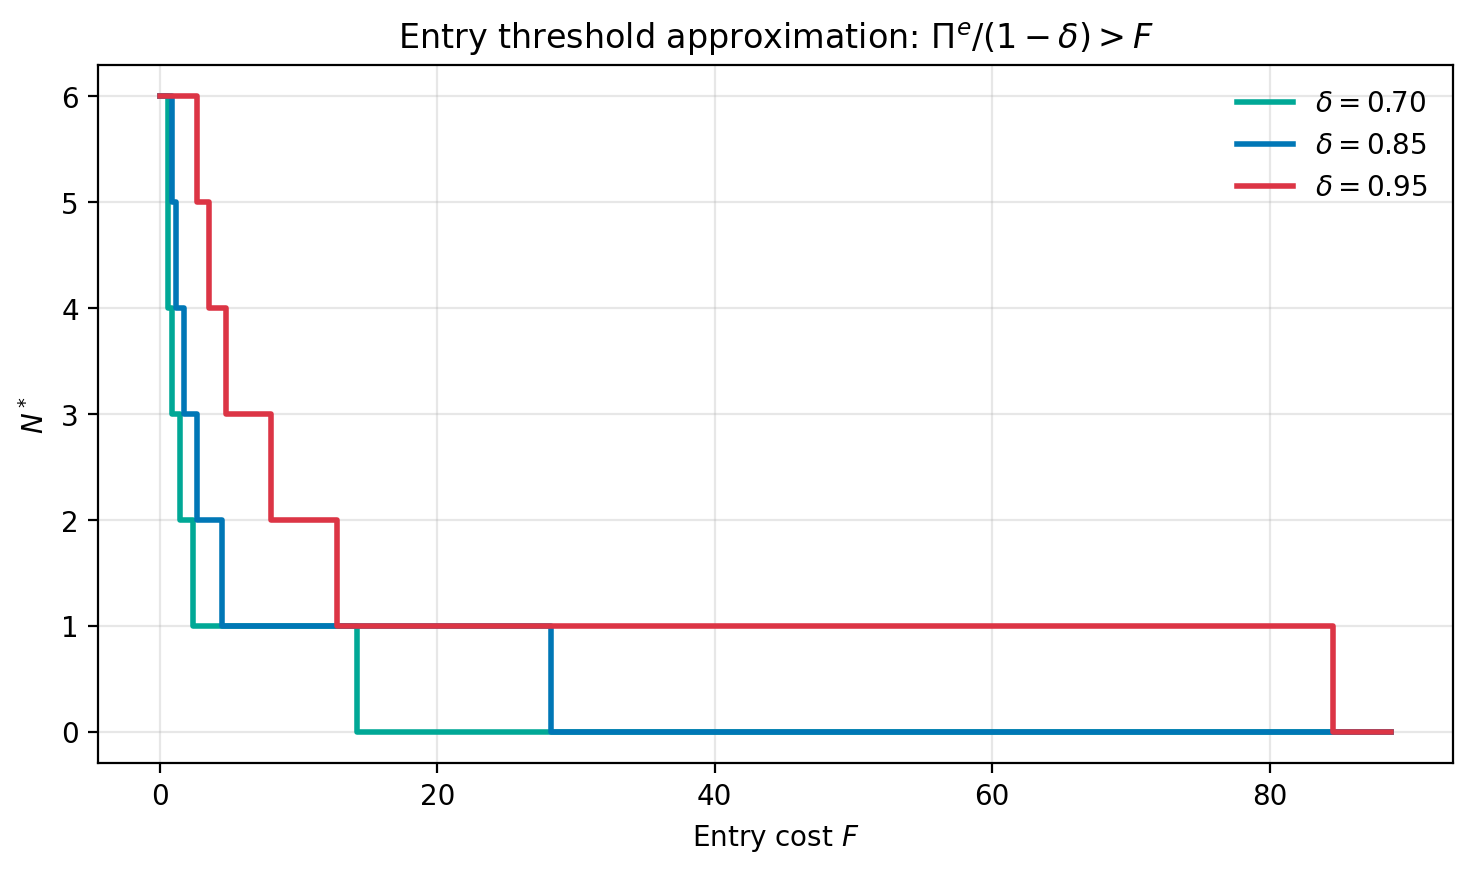
\includegraphics[width=0.75\linewidth]{figures_toy/fig5_nstar_delta.pdf}
  \caption{Illustrative effect of discounting on the entry threshold under the heuristic condition $\Pi^e/(1-\delta)>F$.}
  \label{fig:app_nstar_delta}
\end{figure}

\paragraph{Multiplicity and path dependence}
Figure \ref{fig:app_multiplicity} illustrates how multiple optimal entry locations can arise in symmetric configurations. Starting from the same set of incumbents, different deterministic tie-breaking in the candidate search can lead to distinct final configurations.

\begin{figure}
  \centering
  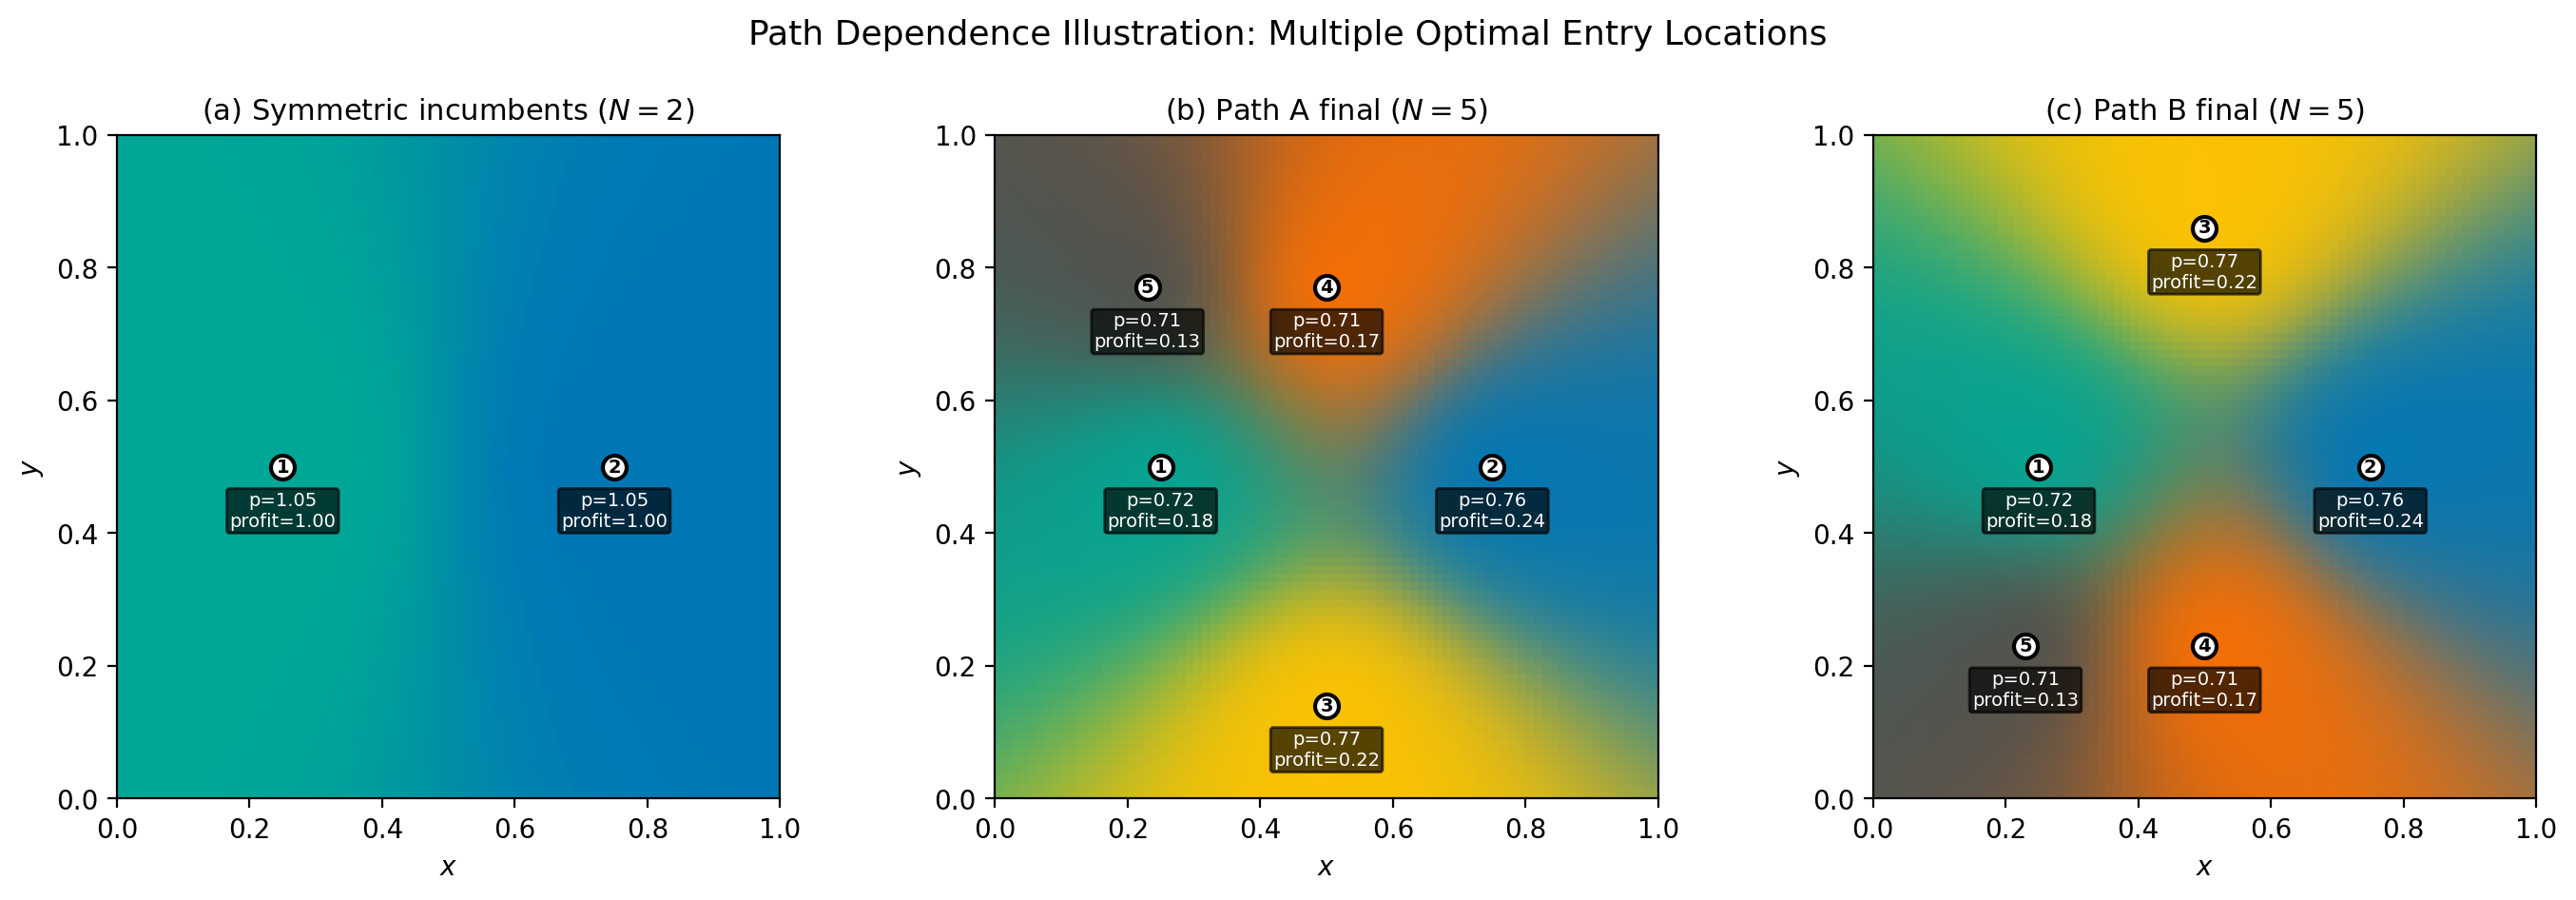
\includegraphics[width=0.95\linewidth]{figures_toy/fig6_multiplicity.pdf}
  \caption{Path dependence illustration (uniform density). Panels (b) and (c) show two distinct final configurations obtained from the same incumbents under different deterministic tie-breaking in the entrant's candidate search.}
  \label{fig:app_multiplicity}
\end{figure}

\subsection{Regularity Diagnostics for Assumption (R)}
\label{app:eta_diagnostics}

Table \ref{tab:eta_diagnostics} reports $\max_i \eta_i(\mathbf{p}^*)$ at the computed equilibrium prices, together with a conservative own-price scan $\eta^{\mathrm{scan}}$ on a one-dimensional grid $p_i\in[c,\overline{p}]$ holding $\mathbf{p}_{-i}=\mathbf{p}_{-i}^*$ fixed. The scan is a diagnostic for numerical regularity and should not be interpreted as a formal test of Assumption \ref{ass:R}, which conditions on interior critical points.

\begin{table}
  \centering
  \begin{threeparttable}
    \caption{Regularity diagnostics for Assumption (R).}
    \label{tab:eta_diagnostics}
    \begin{tabular}{p{0.52\linewidth} c c c}
      \toprule
      Scenario & $N$ & $\max_i \eta_i(\mathbf{p}^*)$ & $\max_i \eta_i^{\mathrm{scan}}$ \\
      \midrule
      Duopoly, uniform, $\beta=5$ & 2 & 0.2513 & 0.9884 \\
      Triopoly, uniform, $\beta=5$ & 3 & 0.5757 & 0.9922 \\
      Entry eq., uniform, $N=6$, $\beta=15$ & 6 & 0.8097 & 1.1255 \\
      Triopoly, uniform, $\beta=50$ (stress test) & 3 & 0.7568 & 2.4116 \\
      Triopoly close, $\beta=50$ (stress test) & 3 & 0.4781 & 1.0000 \\
      \bottomrule
    \end{tabular}
    \begin{tablenotes}[flushleft]
      \footnotesize
    \item Notes: $\eta_i(\mathbf{p}) = \frac{Q_i(\mathbf{p})\,Q_i''(\mathbf{p})}{(Q_i'(\mathbf{p}))^2}$ as defined in Appendix \ref{app:existence_proof}. We define $\eta_i^{\mathrm{scan}} \equiv \max_{p_i\in[c,\overline{p}]} \eta_i(p_i,\mathbf{p}_{-i}^*)$ (computed on a one-dimensional grid), holding rivals fixed at $\mathbf{p}_{-i}^*$. This is a conservative diagnostic and is not a test of Assumption \ref{ass:R} (which conditions on interior critical points and must hold for all $\mathbf{p}_{-i}$). Hence $\eta_i^{\mathrm{scan}} > 2$ does not by itself imply a violation of (R); it indicates that the curvature ratio can exceed $2$ away from critical points in extreme regimes (high $\beta$).
    \end{tablenotes}
  \end{threeparttable}
\end{table}

\section{Extended Proof of Theorem 1: Existence of Price Equilibrium}
\label{app:existence_proof}

We apply Glicksberg's fixed point theorem (1952) to establish existence of a pure-strategy Nash equilibrium.

\paragraph{Compact, Convex Strategy Sets}
Each firm $i \in \mathcal{N}$ chooses $p_i \in [c, \overline{p}]$. This interval is compact and convex. The assumption on $\overline{p}$ is that $\overline{p} < \min_{i,s} (\alpha/\gamma - t \cdot d(s,x_i))$ and $c < \overline{p}$, ensuring $q_i(s) = \alpha - \gamma P_i^*(s) > 0$ for all $s \in S$ and $p_i \in [c, \overline{p}]$.

\paragraph{Continuity of Profit Functions}
$\Pi_i(\mathbf{p}) = (p_i - c)Q_i(\mathbf{p})$. The firm's $i$ demand is $Q_i(\mathbf{p}) = \int_S \rho(s)\,(\alpha - \gamma P_i^*(s))\,\mathrm{Prob}\bigl(i\mid s,\mathbf{p}\bigr)\,ds$. Notice that:
\begin{enumerate}
  \item $P_j^*(s) = p_j + t \cdot d(s,x_j)$ is continuous in $p_j$.
  \item $q_i(s) = \alpha - \gamma P_i^*(s)$ is continuous in $p_i$ (and positive by assumption on $\overline{p}$).
  \item $\mathrm{Prob}(i|s,\mathbf{p}) = \exp(-\beta P_i^*(s)) / \sum_k \exp(-\beta P_k^*(s))$ is continuous in all $p_k$. Denominator is strictly positive.
  \item The integrand $\rho(s)q_i(s)\mathrm{Prob}(i|s,\mathbf{p})$ is continuous in $\mathbf{p}$ and bounded on $S \times [c,\overline{p}]^N$ (since $\rho$ bounded, $q_i(s) \in (0, \alpha]$, $\mathrm{Prob} \in [0,1]$).
  \item By dominated convergence, $Q_i(\mathbf{p})$ is continuous in $\mathbf{p}$.
  \item $\Pi_i(\mathbf{p})$ is continuous as a product of continuous functions.
\end{enumerate}

\paragraph{Quasi-Concavity in Own Price}
Glicksberg's theorem requires each $\Pi_i(\mathbf{p})$ to be quasi-concave in $p_i$. This is imposed in Assumption
\ref{ass:qc}. A sufficient condition can be stated in terms of derivatives of $Q_i$.

Fix firm $i$ and rivals' prices $\mathbf{p}_{-i}$. Write $\Pi_i(p_i,\mathbf{p}_{-i}) = (p_i-c)Q_i(p_i,\mathbf{p}_{-i})$, where
\[
  Q_i(\mathbf{p}) = \int_S \rho(s)\,q_i(s,\mathbf{p})\,L_i(s,\mathbf{p})\,ds,
  \qquad
  q_i(s,\mathbf{p}) = \alpha - \gamma P_i^*(s),
  \qquad
  L_i(s,\mathbf{p}) = \mathrm{Prob}(i\mid s,\mathbf{p}).
\]
Under our assumptions, differentiation under the integral sign is justified. Using $\partial L_i/\partial p_i = -\beta L_i(1-L_i)$ we obtain:
\begin{align*}
  Q_i'(\mathbf{p})
  &= -\int_S \rho(s)\Bigl[\gamma L_i(s,\mathbf{p}) + \beta q_i(s,\mathbf{p})L_i(s,\mathbf{p})(1-L_i(s,\mathbf{p}))\Bigr]ds
  \;<\;0,\\
  Q_i''(\mathbf{p})
  &= \beta\int_S \rho(s)\,L_i(s,\mathbf{p})(1-L_i(s,\mathbf{p}))\Bigl[2\gamma + \beta q_i(s,\mathbf{p})(1-2L_i(s,\mathbf{p}))\Bigr]ds.
\end{align*}

At an interior critical point $\partial \Pi_i(p_i,\mathbf{p}_{-i})/\partial p_i = 0$, we have $p_i-c = -Q_i/Q_i'$, and
\[
  \Pi_i''(p_i,\mathbf{p}_{-i}) = \frac{2(Q_i')^2 - Q_i Q_i''}{Q_i'}.
\]
Since $Q_i'<0$, this critical point is a strict local maximum whenever $2(Q_i')^2 > Q_i Q_i''$. Define the curvature ratio
\[
  \eta_i(\mathbf{p}) \;\equiv\; \frac{Q_i(\mathbf{p})\,Q_i''(\mathbf{p})}{(Q_i'(\mathbf{p}))^2}.
\]
Then the strict second-order condition at any interior critical point is equivalent to $\eta_i(\mathbf{p}) < 2$.

\begin{assumption}[Regularity condition (R)]\label{ass:R}
  For every firm $i$, every $\mathbf{p}_{-i}$, and every interior $p_i\in(c,\overline{p})$ such that
  $\partial \Pi_i(p_i,\mathbf{p}_{-i})/\partial p_i = 0$, we have $\eta_i(p_i,\mathbf{p}_{-i}) < 2$.
\end{assumption}
Under Assumption \ref{ass:R}, every interior critical point of $\Pi_i(\cdot,\mathbf{p}_{-i})$ is a strict local maximum, so
$\Pi_i(\cdot,\mathbf{p}_{-i})$ is quasi-concave on $[c,\overline{p}]$. In particular, Assumption \ref{ass:qc} holds.

\begin{remark}
  In the monopoly case $N=1$, we have $L_1(\cdot,\mathbf{p})\equiv 1$, hence $Q_1''\equiv 0$ and $\eta_1\equiv 0$, so Assumption
  \ref{ass:R} is automatically satisfied.
\end{remark}

\paragraph{Application of Glicksberg's Theorem}
All conditions are met, so at least one pure-strategy Nash equilibrium exists.

\section{Comparative Statics (Proof Sketch)}
\label{app:comparative_statics}

This appendix sketches the proofs for Proposition \ref{prop:comparative} and explains the economics behind each result. A complete sign characterization in full generality requires additional restrictions on primitives (or symmetry): the Jacobian and cross-effects are hard to sign in a general two-dimensional configuration.

\subsection{Preliminaries}

Let $\mathbf{p}^*$ denote the equilibrium price vector. At equilibrium, each firm's first-order condition must be satisfied:
\begin{equation}
  F_i(\mathbf{p}^*) = \frac{\partial \Pi_i(\mathbf{p}^*)}{\partial p_i} = Q_i(\mathbf{p}^*) + (p_i^* - c)\frac{\partial Q_i(\mathbf{p}^*)}{\partial p_i} = 0 \quad \forall i \in \mathcal{N}
\end{equation}

To analyze how equilibrium prices change with respect to a parameter $\theta \in \{\beta, \gamma, t, \alpha\}$, we apply the implicit function theorem to the system of equations $F_i(\mathbf{p}^*,\theta) = 0$. Define the Jacobian matrix $J = [\frac{\partial F_i}{\partial p_j}]_{i,j}$. The changes in equilibrium prices with respect to $\theta$ are given by:
\begin{equation}
  \frac{d\mathbf{p}^*}{d\theta} = -J^{-1}\cdot\frac{\partial \mathbf{F}}{\partial \theta}
\end{equation}

where $\frac{\partial \mathbf{F}}{\partial \theta} = [\frac{\partial F_i}{\partial \theta}]_i$ is the vector of partial derivatives with respect to $\theta$.

Under conditions where the Jacobian $J$ is invertible, and if all elements of $\frac{\partial \mathbf{F}}{\partial \theta}$ have the same sign, and the off-diagonal elements of $-J^{-1}$ are non-negative, the corresponding elements of $\frac{d\mathbf{p}^*}{d\theta}$ will have the same sign as $-\frac{\partial F_i}{\partial \theta}$. This allows us to determine the direction of price changes.

\subsection{Effects of Changing $\beta$ (Choice Intensity)}

For the choice intensity parameter $\beta$, we have:
\begin{equation}
  \frac{\partial F_i}{\partial \beta} = \frac{\partial Q_i}{\partial \beta} + (p_i^* - c)\frac{\partial^2 Q_i}{\partial p_i \partial \beta}
\end{equation}

As $\beta$ increases, consumers become more price-sensitive, making $\frac{\partial Q_i}{\partial p_i}$ more negative. This increased elasticity pushes firms to reduce prices.

At equilibrium, this effect typically dominates:
\begin{equation}
  \frac{\partial F_i}{\partial \beta} < 0
\end{equation}

If so for all $i$:
\begin{equation}
  \frac{dp_i^*}{d\beta} < 0
\end{equation}

\subsection{Effects of Changing $\gamma$ (Price Sensitivity)}

For the demand price sensitivity parameter $\gamma$, we have:
\begin{equation}
  \frac{\partial F_i}{\partial \gamma} = \frac{\partial Q_i}{\partial \gamma} + (p_i^* - c)\frac{\partial^2 Q_i}{\partial p_i \partial \gamma}
\end{equation}

As $\gamma$ increases, each consumer's quantity demanded falls for a given effective price; demand also becomes more price-responsive.

Both effects push in the same direction:
\begin{equation}
  \frac{\partial F_i}{\partial \gamma} < 0
\end{equation}

Under the same condition:
\begin{equation}
  \frac{dp_i^*}{d\gamma} < 0
\end{equation}

\subsection{Effects of Changing $t$ (Transportation Cost)}

As $t$ increases, spatial differentiation becomes more important relative to price differences, so demand becomes less price-elastic. This is the dominant effect:
\begin{equation}
  \frac{\partial F_i}{\partial t} > 0
\end{equation}

Then:
\begin{equation}
  \frac{dp_i^*}{dt} > 0
\end{equation}

\subsection{Effects of Changing $\alpha$ (Base Demand)}

Higher $\alpha$ raises quantity demanded proportionally across all firms:
\begin{equation}
  \frac{\partial F_i}{\partial \alpha} > 0
\end{equation}

Hence:
\begin{equation}
  \frac{dp_i^*}{d\alpha} > 0
\end{equation}

\section{Analysis of Dynamic Entry Game}
\label{app:dynamic_entry}

This appendix proves the existence results for the dynamic entry game stated in Section \ref{sec:dynamic} and explains why multiple equilibria typically arise.

\subsection{Proof of Theorem \ref{thm:existence_entry}: Existence of SPNE}

The proof proceeds in three steps:

\subsubsection*{Step 1: Bounded Number of Firms}

We first establish that the entry process eventually terminates at some finite number of firms.

\begin{lemma}[Bounded Entry]
  There exists a finite upper bound $\bar{N}$ such that if $N_\tau \geq \bar{N}$, no further entry will occur in any SPNE.
\end{lemma}

\begin{proof}
  Fix any number of firms $N\ge 1$, any location configuration $\mathbf{x}_N$, and any price vector $\mathbf{p}\in[c,\overline{p}]^N$.
  For each $s\in S$ and each $i\in\{1,\ldots,N\}$, the effective price satisfies
  $c \le P_i^*(s) \le \overline{p} + t\overline{d}$, where $\overline{d}=\max_{s,x\in S} d(s,x)$.
  Hence the logit share obeys the uniform bound
  \[
    L_i(s,\mathbf{p})
    \;=\;
    \frac{\exp(-\beta P_i^*(s))}{\sum_{j=1}^N \exp(-\beta P_j^*(s))}
    \;\le\;
    \frac{\exp(-\beta c)}{N\,\exp(-\beta(\overline{p}+t\overline{d}))}
    \;=\;
    \frac{K}{N},
  \]
  where $K\equiv \exp(\beta(\overline{p}+t\overline{d}-c))$ is finite and independent of $N$ and $\mathbf{x}_N$.

  Moreover, individual demand satisfies $q_i(s,\mathbf{p})=\alpha-\gamma P_i^*(s)\le \alpha-\gamma c$.
  Therefore,
  \[
    Q_i(\mathbf{p})
    \;=\;
    \int_S \rho(s)\,q_i(s,\mathbf{p})\,L_i(s,\mathbf{p})\,ds
    \;\le\;
    (\alpha-\gamma c)\,M\,\frac{K}{N},
  \]
  and for each firm $i$,
  \[
    \Pi_i(\mathbf{p})
    \;=\;
    (p_i-c)\,Q_i(\mathbf{p})
    \;\le\;
    (\overline{p}-c)\,(\alpha-\gamma c)\,M\,\frac{K}{N}
    \;=\;
    \frac{C}{N},
  \]
  where $C\equiv (\overline{p}-c)(\alpha-\gamma c)MK$.

  Consider now an entry stage with $N$ incumbents. If a new firm enters, the subsequent price subgame has $N+1$ firms, so its one-period equilibrium profit is bounded above by $C/(N+1)$.
  Since $N$ can only increase over time, its continuation value from entry is bounded by the perpetuity $C/((N+1)(1-\delta))$.
  Choose
  \[
    \bar{N}
    \;\equiv\;
    \left\lceil \frac{C}{F(1-\delta)} \right\rceil + 1.
  \]
  Then for every $N\ge \bar{N}$, any entrant's continuation value is strictly below $F$, so entry is unprofitable. Therefore, no further entry occurs once $N_\tau\ge \bar{N}$.
\end{proof}

\subsubsection*{Step 2: Existence of Optimal Strategies at Each Stage}

\begin{lemma}[Price Equilibrium Existence]
  For any number of firms $N$ and location configuration $\mathbf{x}_N$, a pure-strategy Nash equilibrium of the price-setting game exists.
\end{lemma}

\begin{proof}
  This follows directly from Theorem \ref{thm:existence}. The price-setting game satisfies the conditions of Glicksberg's theorem.
\end{proof}

\begin{lemma}[Optimal Location Choice]
  For any configuration of incumbent firms $\mathbf{x}_{inc}$, if entry is profitable, there exists an optimal location choice for the entrant.
\end{lemma}

\begin{proof}
  Fix incumbents' locations $\mathbf{x}_{inc}$ with $N$ firms. For each prospective entrant location $x_E\in S$, consider the $(N+1)$-firm price subgame with location vector $(\mathbf{x}_{inc},x_E)$, and let $\mathcal{E}(\mathbf{x}_{inc},x_E)\subset[c,\overline{p}]^{N+1}$ denote its set of Nash equilibria.
  By Theorem \ref{thm:existence}, $\mathcal{E}(\mathbf{x}_{inc},x_E)$ is non-empty for every $x_E$; it is compact because it is a closed subset of the compact set $[c,\overline{p}]^{N+1}$.
  Moreover, $\mathcal{E}(\mathbf{x}_{inc},\cdot)$ has a closed graph (equilibrium conditions are preserved under limits by continuity of payoffs), so it is upper hemi-continuous.

  Define the entrant's equilibrium-profit value function as the maximum profit over price equilibria,
  \[
    V_E(\mathbf{x}_{inc},x_E)
    \;\equiv\;
    \max_{\mathbf{p}\in\mathcal{E}(\mathbf{x}_{inc},x_E)}
    \Pi_{N+1}\bigl(\mathbf{p};\mathbf{x}_{inc},x_E\bigr).
  \]
  The profit function $\Pi_{N+1}(\mathbf{p};\mathbf{x}_{inc},x_E)$ is continuous in $(\mathbf{p},x_E)$ by dominated convergence (the integrand is continuous in distances and uniformly bounded on $S\times[c,\overline{p}]^{N+1}$).
  Berge's maximum theorem then implies that $V_E(\mathbf{x}_{inc},\cdot)$ is upper semi-continuous and attains a maximum on the compact set $S$.
  Hence there exists an optimal entrant location $x_E^*\in\arg\max_{x_E\in S} V_E(\mathbf{x}_{inc},x_E)$.
\end{proof}

\subsubsection*{Step 3: Construction of SPNE}

We construct an SPNE by backward induction on the number of incumbents, using the upper bound $\bar{N}$ from Lemma 1.

\paragraph{Terminal case ($N\ge \bar{N}$).}
By Lemma 1, when $N\ge \bar{N}$ no further entrant can recoup the fixed cost, so ``do not enter'' is optimal in every entry subgame.
In every price subgame, a Nash equilibrium exists by Theorem \ref{thm:existence}; playing a Nash equilibrium in each price subgame is sequentially rational.
Therefore an SPNE exists for every subgame with $N\ge \bar{N}$ incumbents.

\paragraph{Inductive step.}
Fix $N<\bar{N}$ and suppose that for every location configuration $\mathbf{x}_{N+1}$ there exists an SPNE of the continuation game starting from the next entry stage with $N+1$ incumbents.
Consider any subgame that begins at an entry stage with $N$ incumbents located at $\mathbf{x}_N$.
If the potential entrant stays out, its payoff is $0$.
If it enters and chooses $x_E\in S$, the subsequent price subgame has $N+1$ firms and admits a Nash equilibrium by Theorem \ref{thm:existence}; thereafter, play follows an SPNE of the continuation game by the inductive hypothesis.
Let $W_E(\mathbf{x}_N,x_E)$ denote the entrant's continuation value from entering at $x_E$ (net of the fixed cost $F$) under this continuation play.
By Assumption \ref{ass:entry_values} and compactness of $S$, the set of optimal entry locations
$X_E^*(\mathbf{x}_N)\equiv \arg\max_{x_E \in S} W_E(\mathbf{x}_N, x_E)$ is non-empty.
To complete the strategy definition, we employ a deterministic tie-breaking rule (e.g., lexicographic selection) to select a unique $x_E^* \in X_E^*(\mathbf{x}_N)$.
The strategy profile is then: the entrant enters at $x_E^*$ if $W_E(\mathbf{x}_N, x_E^*) > 0$ (and stays out otherwise); if entry occurs, play proceeds according to the inductively defined SPNE. This construction satisfies sequential rationality at the entry stage and, by hypothesis, in all subsequent subgames.

Combining these strategies yields an SPNE for the subgame with $N$ incumbents.
By induction, an SPNE exists starting from the initial empty market.

\subsection{Proof of Theorem \ref{thm:non_uniqueness_entry}: Multiplicity of Equilibria}

We now explain why multiple SPNE typically exist. The argument is constructive: we exhibit three independent sources of multiplicity.

\subsubsection*{Source 1: Multiple Optimal Locations}

\begin{lemma}[Location Multiplicity]
  There exist market configurations where an entrant has multiple optimal locations that yield equivalent profits.
\end{lemma}

\begin{proof}
  Consider a symmetric case with $\rho(s)$ uniform on a disc $S$, and two incumbents located at opposite sides of the disc's circumference. By symmetry, a third entrant has at least two optimal locations that yield identical profits. Each of these location choices leads to a different market configuration and affects the entry decisions and optimal locations for subsequent entrants.
\end{proof}

\subsubsection*{Source 2: Path Dependence}

\begin{lemma}[Path Dependence]
  Different sequences of entry decisions can lead to different equilibrium market structures.
\end{lemma}

\begin{proof}
  Let $\mathbf{x}_A = (x_1^A, x_2^A, \ldots, x_{N_A}^A)$ and $\mathbf{x}_B = (x_1^B, x_2^B, \ldots, x_{N_B}^B)$ be two different location configurations reached through different entry sequences. Because locations affect equilibrium profits, the continuation value of entry $\max_{x_E\in S} W_E(\mathbf{x},x_E)$ can differ across configurations. It is therefore possible that $\max_{x_E\in S} W_E(\mathbf{x}_A,x_E) > 0$ while $\max_{x_E\in S} W_E(\mathbf{x}_B,x_E) < 0$, meaning entry continues in path A but stops in path B. This leads to equilibria with different numbers of firms.
\end{proof}

These sources of multiplicity establish that the entry-location-price game typically admits multiple SPNE, completing the proof of Theorem \ref{thm:non_uniqueness_entry}.

\subsection{Market Structure Properties}

We now provide the reasoning for the comparative statics on market structure presented in Proposition \ref{prop:market_structure}.

\begin{proposition}[Entry Cost Effect]
  The equilibrium number of firms $N^*$ is non-increasing in the entry cost $F$.
\end{proposition}

\begin{proof}
  Entry occurs in an entry subgame if and only if $\max_{x_E\in S} W_E(\mathbf{x}_{N-1},x_E) > 0$, where the fixed cost enters the continuation value subtractively. Increasing $F$ weakly decreases $W_E$ in every subgame, which cannot increase the number of firms that enter in equilibrium.
\end{proof}

\begin{proposition}[Market Size Effect]
  The equilibrium number of firms $N^*$ is non-decreasing in the market size $M = \int_S \rho(s) ds$.
\end{proposition}

\begin{proof}
  A proportional increase in $\rho(s)$ across all locations increases per-period demands and profits proportionally. This raises entrants' continuation values $W_E$, so entry becomes more likely for a given number of incumbents and equilibrium market size may increase.
\end{proof}

\begin{proposition}[Competition Parameters]
  The equilibrium number of firms $N^*$ is:
  \begin{enumerate}
    \item Non-increasing in $\beta$ (choice intensity parameter)
    \item Non-increasing in $\gamma$ (demand price sensitivity)
    \item Non-decreasing in $t$ (transportation cost parameter)
  \end{enumerate}
\end{proposition}

\begin{proof}
  From Section \ref{app:comparative_statics}, the comparative statics discussion suggests that:
  \begin{itemize}
    \item Higher $\beta$ and $\gamma$ intensify price competition, reducing equilibrium prices and profits
    \item Higher $t$ softens price competition, increasing equilibrium prices and profits
  \end{itemize}

  Since the entry decision is based on the sign of $\max_{x_E\in S} W_E(\mathbf{x}_{N-1},x_E)$, lower profits make entry harder to justify, while higher profits make it easier. The effects on $N^*$ follow accordingly.
\end{proof}
\bibliography{bibliography}
\end{document}
